%%%%%%%%%%%%%%%%%%%%%%%%%%%%%%%%%%%%%%%%%
% Beamer Presentation
% LaTeX Template
% Version 1.0 (10/11/12)
%
% This template has been downloaded from:
% http://www.LaTeXTemplates.com
%
% License:
% CC BY-NC-SA 3.0 (http://creativecommons.org/licenses/by-nc-sa/3.0/)
%
%%%%%%%%%%%%%%%%%%%%%%%%%%%%%%%%%%%%%%%%%

%----------------------------------------------------------------------------------------
%	PACKAGES AND THEMES
%----------------------------------------------------------------------------------------

\documentclass{beamer}
\usepackage{hyperref} 
\hypersetup{%
    pdfencoding=auto,
    pdfauthor={Kyunghoon Kim},
    pdftitle={NetworkX를 이용한 네트워크 분석}
    }
\mode<presentation> {

% The Beamer class comes with a number of default slide themes
% which change the colors and layouts of slides. Below this is a list
% of all the themes, uncomment each in turn to see what they look like.
\usepackage[utf8]{inputenc}
%\usepackage{minted}
%\usetheme{default}
%\usetheme{AnnArbor}
%\usetheme{Antibes}
%\usetheme{Bergen}
%\usetheme{Berkeley}
%\usetheme{Berlin}
%\usetheme{Boadilla}
%\usetheme{CambridgeUS}
%\usetheme{Copenhagen}
%\usetheme{Darmstadt}
%\usetheme{Dresden}
%\usetheme{Frankfurt}
%\usetheme{Goettingen}
%\usetheme{Hannover}
%\usetheme{Ilmenau}
%\usetheme{JuanLesPins}
%\usetheme{Luebeck}
\usetheme{Madrid} % %
%\usetheme{Malmoe}
%\usetheme{Marburg}
%\usetheme{Montpellier}
%\usetheme{PaloAlto}
%\usetheme{Pittsburgh}
%\usetheme{Rochester}
%\usetheme{Singapore}
%\usetheme{Szeged}
%\usetheme{Warsaw}

% As well as themes, the Beamer class has a number of color themes
% for any slide theme. Uncomment each of these in turn to see how it
% changes the colors of your current slide theme.

%\usecolortheme{albatross}
%\usecolortheme{beaver}
%\usecolortheme{beetle}
%\usecolortheme{crane}
%\usecolortheme{dolphin}
%\usecolortheme{dove}
%\usecolortheme{fly}
%\usecolortheme{lily}
%\usecolortheme{orchid}
%\usecolortheme{rose}
%\usecolortheme{seagull}
%\usecolortheme{seahorse}
%\usecolortheme{whale}
%\usecolortheme{wolverine}

%\setbeamertemplate{footline} % To remove the footer line in all slides uncomment this line
%\setbeamertemplate{footline}[page number] % To replace the footer line in all slides with a simple slide count uncomment this line

%\setbeamertemplate{navigation symbols}{} % To remove the navigation symbols from the bottom of all slides uncomment this line
} %set beamer

%\usepackage{kotex}
\usepackage[cjk,hangul]{kotex}
\newcommand{\fbckg}[1]{\usebackgroundtemplate{\includegraphics[width=\paperwidth]{#1}}}%frame background
\graphicspath{{./}} % Location of the slide background and figure files
\usepackage{graphicx} % Allows including images
\usepackage{booktabs} % Allows the use of \toprule, \midrule and \bottomrule in tables
%\usepackage{python}
%\usebackgroundtemplate{\includegraphics[width=\paperwidth,height=\paperheight]{a.png}}
%\usepackage[usenames,dvipsnames]{color}
\usepackage{color}
%\usepackage{xcolor}
%\usepackage{fancyvrb}
%\usepackage[usenames,dvipsnames]{xcolor}
%\fvset{frame=single,framesep=1mm,fontfamily=courier,fontsize=\scriptsize,numbers=left,framerule=.3mm,numbersep=1mm,commandchars=\\\{\}}
\usepackage{fancyvrb,xcolor}% http://ctan.org/pkg/{fancyvrb,xcolor}
\DefineVerbatimEnvironment%
  {CodeVerbatim}{Verbatim}
  {formatcom=\color{red}}

%%%%%%%%%%%%%%%%
% PYTHON STYLE
%\usepackage{color}
%\usepackage{listings}
%\usepackage{setspace}
%
%\definecolor{Code}{rgb}{0,0,0}
%\definecolor{Decorators}{rgb}{0.5,0.5,0.5}
%\definecolor{Numbers}{rgb}{0.5,0,0}
%\definecolor{MatchingBrackets}{rgb}{0.25,0.5,0.5}
%\definecolor{Keywords}{rgb}{0,0,1}
%\definecolor{self}{rgb}{0,0,0}
%\definecolor{Strings}{rgb}{0,0.63,0}
%\definecolor{Comments}{rgb}{0,0.63,1}
%\definecolor{Backquotes}{rgb}{0,0,0}
%\definecolor{Classname}{rgb}{0,0,0}
%\definecolor{FunctionName}{rgb}{0,0,0}
%\definecolor{Operators}{rgb}{0,0,0}
%\definecolor{Background}{rgb}{0.98,0.98,0.98}
%
%\lstnewenvironment{pythoncode}[1][]{
%\lstset{
%numbers=left,
%numberstyle=\footnotesize,
%numbersep=1em,
%xleftmargin=1em,
%framextopmargin=2em,
%framexbottommargin=2em,
%showspaces=false,
%showtabs=false,
%showstringspaces=false,
%frame=l,
%tabsize=4,
%% Basic
%basicstyle=\ttfamily\small\setstretch{1},
%backgroundcolor=\color{Background},
%language=Python,
%% Comments
%commentstyle=\color{Comments}\slshape,
%% Strings
%stringstyle=\color{Strings},
%morecomment=[s][\color{Strings}]{"""}{"""},
%morecomment=[s][\color{Strings}]{'''}{'''},
%% keywords
%morekeywords={import,from,class,def,for,while,if,is,in,elif,else,not,and,or,print,break,continue,return,True,False,None,access,as,,del,except,exec,finally,global,import,lambda,pass,print,raise,try,assert},
%keywordstyle={\color{Keywords}\bfseries},
%% additional keywords
%morekeywords={[2]@invariant},
%keywordstyle={[2]\color{Decorators}\slshape},
%emph={self},
%emphstyle={\color{self}\slshape},
%}}{}


%http://tex.stackexchange.com/questions/85269/easy-absolute-positioning-in-beamer
\usepackage{tikz}
\def\mytemparray{}
\newcommand\doatpos[3]{%
    \bgroup
    \def\mytemparray{{ #2 }}
    \pgfmathparse{\mytemparray[0]} \edef\mya{\pgfmathresult}
    \pgfmathparse{\mytemparray[1]} \edef\myb{\pgfmathresult}
    \pgfmathparse{\mytemparray[2]} \edef\myc{\pgfmathresult} %also possible \pgfmathsetmacro
    \begin{tikzpicture}[remember picture, overlay]
            \node[anchor=#1, opacity=\myc] at ( \mya pt, \myb  pt) {#3};
    \end{tikzpicture}%
        %
    %
    \egroup
%
}

%----------------------------------------------------------------------------------------
%	TITLE PAGE
%----------------------------------------------------------------------------------------
\title[NetworkX with Network Analysis]{NetworkX를 이용한 네트워크 분석} % The short title appears at the bottom of every slide, the full title is only on the title pag석

\author{김경훈} % Your name
\institute[UNIST] % Your institution as it will appear on the bottom of every slide, may be shorthand to save space
{
유니스트 수리과학과\\ % Your institution for the title page
\medskip
\textit{kyunghoon@unist.ac.kr} % Your email address
}
%\date{\today} % Date, can be changed to a custom date
\date{2014년 8월 30일}

\begin{document}
{
%\usebackgroundtemplate{\includegraphics[width=\paperwidth]{a.png}}%
%\fbckg{Untitled.png}
\fbckg{cover.png}
\begin{frame}
\doatpos{west}{4.05cm, -5.4cm,.7}{\scriptsize{숙명여자대학교 창학관 젬마홀}}
\titlepage % Print the title page as the first slide
\begin{center}
\href{http://www.pycon.kr/}{
\includegraphics[scale=0.3]{pycon.png}}
\end{center}
\end{frame}
}

\begin{frame}
\frametitle{이번 TALK의 목적}
\begin{enumerate}
\item LaTeX\\

\includegraphics[scale=0.2]{donald.png}
\quad
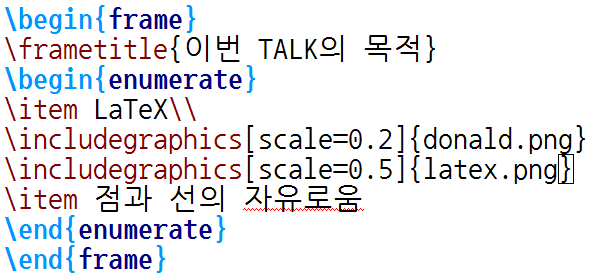
\includegraphics[scale=0.5]{latex.png}\\
\item 점과 선의 자유로움\\
\item 파이썬이라서 자유로운 점
\end{enumerate}
\end{frame}

\begin{frame}
\frametitle{About me}
\textbf{Speak{\textcolor{blue}{er}}}\\
\href{https://www.linkedin.com/pub/kyunghoon-kim/44/889/69a}{김경훈} (대학원생)\\
UNIST (Ulsan National Institute of Science and Technology)\\
\href{http://math.unist.ac.kr}{자연과학부 수리과학과}\\
\textbf{{\textcolor{blue}{Lab}}}\\
Adviser : \href{https://www.linkedin.com/pub/bongsoo-jang/63/829/197}{Bongsoo Jang}\\
Homepage : \href{http://amath.unist.ac.kr}{http://amath.unist.ac.kr}\\
\begin{center}

\includegraphics[scale=0.35]{unist.jpg}\\
\tiny{``Be the light that shines the world with science and technology.''}
\end{center}
\end{frame}

\begin{frame}
\frametitle{목차} % Table of contents slide, comment this block out to remove it
\tableofcontents % Throughout your presentation, if you choose to use \section{} and \subsection{} commands, these will automatically be printed on this slide as an overview of your presentation
\end{frame}

%----------------------------------------------------------------------------------------
%	PRESENTATION SLIDES
%----------------------------------------------------------------------------------------

\section{네트워크?}
\begin{frame}
\frametitle{네트워크?}
\textbf{데이터 추상화}\\
\begin{center}

\includegraphics[scale=0.3]{applepear.png}
\end{center}
\end{frame}

\begin{frame}
\frametitle{네트워크?}
\textbf{데이터 추상화}\\
\begin{center}

\includegraphics[scale=0.3]{android.png}
\end{center}
\end{frame}

\begin{frame}
\frametitle{네트워크?}
\textbf{데이터 추상화}\\
\begin{center}
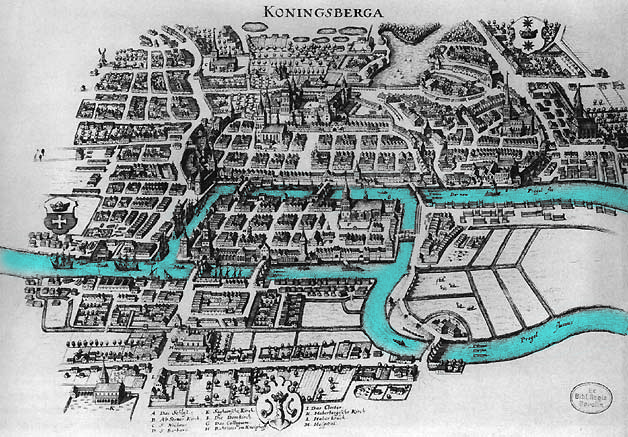
\includegraphics[scale=0.35]{Koenigsberg.jpg}
\end{center}
\hfill
\tiny
\href{http://en.wikipedia.org/wiki/K\%C3\%B6nigsberg}{http://en.wikipedia.org/wiki/K\%C3\%B6nigsberg}
\end{frame}

\begin{frame}
\frametitle{네트워크?}
\textbf{데이터 추상화}\\
\begin{center}
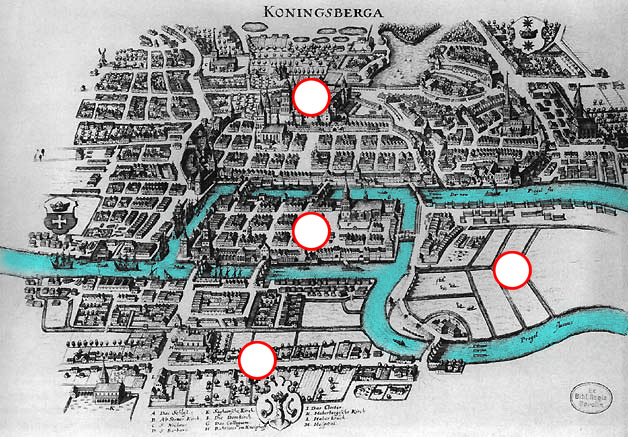
\includegraphics[scale=0.35]{Koenigsberg_node.jpg}
\end{center}
\hfill
\tiny
\href{http://en.wikipedia.org/wiki/K\%C3\%B6nigsberg}{http://en.wikipedia.org/wiki/K\%C3\%B6nigsberg}
\end{frame}

\begin{frame}
\frametitle{네트워크?}
\textbf{데이터 추상화}\\
\begin{center}
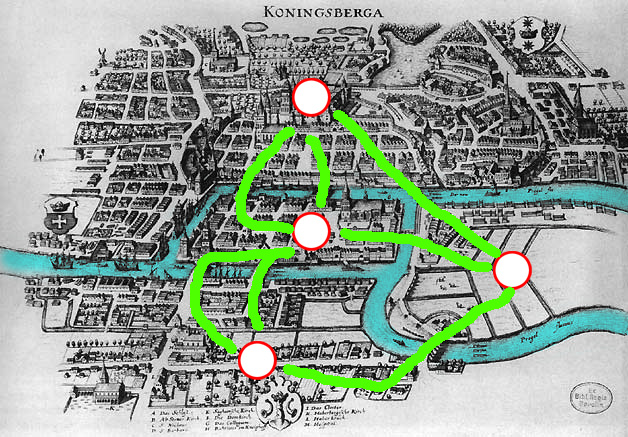
\includegraphics[scale=0.35]{Koenigsberg_edge.jpg}
\end{center}
\hfill
\tiny
\href{http://en.wikipedia.org/wiki/K\%C3\%B6nigsberg}{http://en.wikipedia.org/wiki/K\%C3\%B6nigsberg}
\end{frame}

\begin{frame}
\frametitle{네트워크?}
\textbf{데이터 추상화}\\
\begin{center}
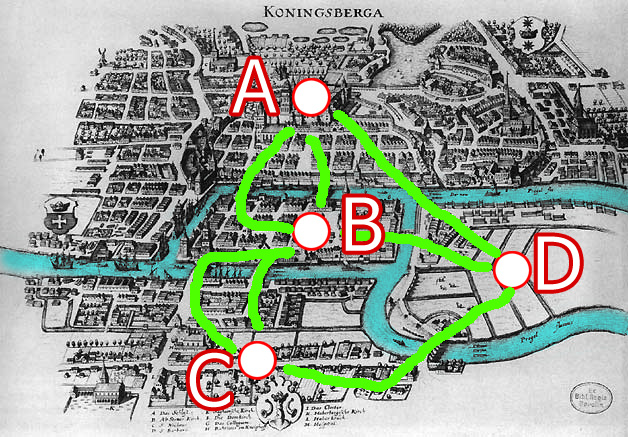
\includegraphics[scale=0.35]{Koenigsberg_symbol.jpg}
\end{center}
\hfill
\tiny
\href{http://en.wikipedia.org/wiki/K\%C3\%B6nigsberg}{http://en.wikipedia.org/wiki/K\%C3\%B6nigsberg}
\end{frame}

\begin{frame}
\frametitle{네트워크?}
\textbf{데이터 추상화}\\
\begin{center}
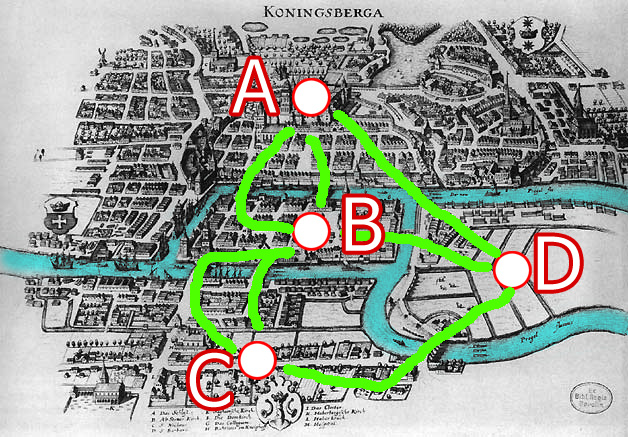
\includegraphics[scale=0.3]{Koenigsberg_symbol.jpg}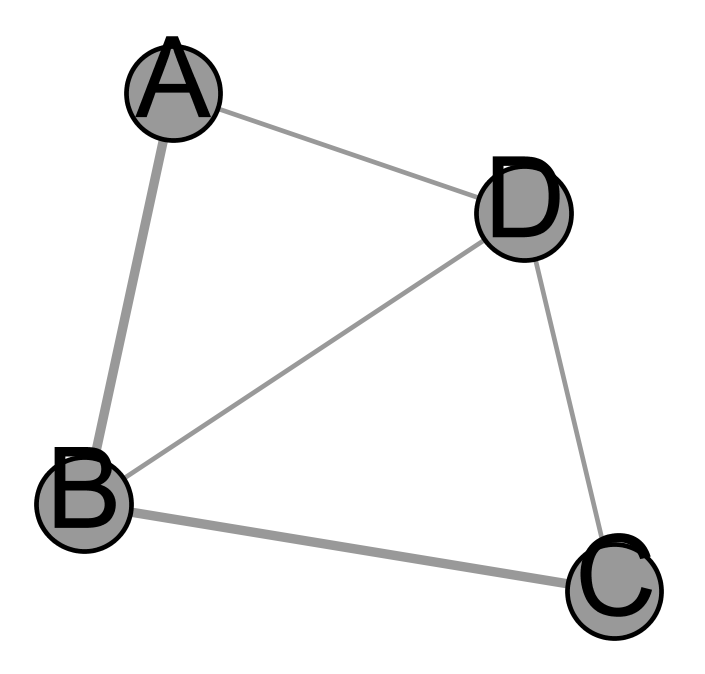
\includegraphics[scale=0.3]{Koenigsberg.png}
\end{center}
\end{frame}

\begin{frame}[fragile]
\frametitle{네트워크?}
\begin{verbatim}
>>> G = nx.MultiGraph()
>>> G.add_nodes_from([`A',`B',`C',`D'])
>>> G.add_edges_from([(`A',`B'),(`A',`B'),(`A',`D'),(`B',`D')
,(`B',`C'),(`B',`C'),(`C',`D')])
>>> nx.draw(G)
>>> plt.show()
\end{verbatim}
\end{frame}

\begin{frame}
\frametitle{네트워크?}
\begin{table}
\begin{tabular}{l | l l}
\toprule
\textbf{네트워크} & \textbf{노드}(Node) & \textbf{엣지}(Edge)\\
\midrule
인터넷 네트워크 & 컴퓨터 & 케이블 \\
월드와이드웹 & 웹 페이지 & 하이퍼링크 \\
인용 네트워크 & 글 & 인용 \\
전력망 & 발전기 & 전선 \\
친구 네트워크 & 사람 & 친구관계 \\
신진대사 네트워크 & 대사 산물 & 반응 \\
신경망 & 뉴런 & 시냅스 \\
먹이사슬 네트워크 & 종 & 포식 \\
\bottomrule
\end{tabular}
\caption{네트워크 예제}
\end{table}
\end{frame}
%본 슬라이드에서의 네트워크는 수학에서 말하는 그래프와 동일합니다.

{
\fbckg{networkx.png}
\begin{frame}
\frametitle{NetworkX : Python Library}
NetworkX is a Python language software package for the creation, manipulation, and study of the structure, dynamics, and functions of complex networks.

\textbf{Features}
\begin{enumerate}
\item 무방향성, 방향성, 다중그래프 등의 데이터 구조
\item Nodes can be "anything" (e.g. text, images, XML records)
\item Edges can hold arbitrary data (e.g. weights, time-series)
\item 표준적인 그래프 알고리즘.
\item BSD 라이센스
\item Well tested: more than 1800 unit tests
\item PYTHON LIBRARY!
\end{enumerate}
\end{frame}
}

\begin{frame}
\frametitle{NetworkX 설치방법}
\begin{itemize}
\item 수동 설치 \hfill \\
\href{https://pypi.python.org/pypi/networkx/}{https://pypi.python.org/pypi/networkx/}
\item 자동 설치 \hfill \\
easy\_install networkx\\
pip install networkx\\
sudo apt-get install python-networkx
\item 통합 설치 \hfill \\
\href{https://www.enthought.com/products/canopy/}{Enthought Canopy}\\
\href{https://store.continuum.io/}{Continuum Analytics Anaconda}\\
\href{https://code.google.com/p/pythonxy/}{Python(x,y)}\\
\href{https://code.google.com/p/winpython/}{WinPython}
\end{itemize}
\end{frame}
% 직접 하나하나 셋팅하는 것도 좋지만, matplotlib 등 다른 라이브러리도 설치해야 하는 불편함 때문에 통합 설치를 하는 것도 나쁘지 않다.

\begin{frame}[fragile] % Need to use the fragile option when verbatim is used in the slide
\frametitle{네트워크의 간단한 예}
%[commandchars=\\\{\}],formatcom=\color{red}
\begin{Verbatim}[numbers=left,commandchars=\\\{\}]
>>> import networkx as nx \textcolor{red}{% 라이브러리를 nx로 불러오기}
\end{Verbatim}
\end{frame}

\begin{frame}[fragile] % Need to use the fragile option when verbatim is used in the slide
\frametitle{네트워크의 간단한 예}
%[commandchars=\\\{\}],formatcom=\color{red}
\begin{Verbatim}[numbers=left,commandchars=\\\{\}]
>>> import networkx as nx \textcolor{red}{% 라이브러리를 nx로 불러오기}
>>> import matplotlib.pyplot as plt \textcolor{red}{% plt로 불러오기}
\end{Verbatim}
\end{frame}

\begin{frame}[fragile] % Need to use the fragile option when verbatim is used in the slide
\frametitle{네트워크의 간단한 예}
%[commandchars=\\\{\}],formatcom=\color{red}
\begin{Verbatim}[numbers=left,commandchars=\\\{\}]
>>> import networkx as nx \textcolor{red}{% 라이브러리를 nx로 불러오기}
>>> import matplotlib.pyplot as plt \textcolor{red}{% plt로 불러오기}
>>> G = nx.Graph() \textcolor{red}{% 빈 그래프 구조 G 생성}
\end{Verbatim}
\end{frame}

\begin{frame}[fragile] % Need to use the fragile option when verbatim is used in the slide
\frametitle{네트워크의 간단한 예}
%[commandchars=\\\{\}],formatcom=\color{red}
\begin{Verbatim}[numbers=left,commandchars=\\\{\}]
>>> import networkx as nx \textcolor{red}{% 라이브러리를 nx로 불러오기}
>>> import matplotlib.pyplot as plt \textcolor{red}{% plt로 불러오기}
>>> G = nx.Graph() \textcolor{red}{% 빈 그래프 구조 G 생성}
>>> G.add_edge(1,2) \textcolor{red}{% 엣지 추가}
\end{Verbatim}
\end{frame}

\begin{frame}[fragile] % Need to use the fragile option when verbatim is used in the slide
\frametitle{네트워크의 간단한 예}
%[commandchars=\\\{\}],formatcom=\color{red}
\begin{Verbatim}[numbers=left,commandchars=\\\{\}]
>>> import networkx as nx \textcolor{red}{% 라이브러리를 nx로 불러오기}
>>> import matplotlib.pyplot as plt \textcolor{red}{% plt로 불러오기}
>>> G = nx.Graph() \textcolor{red}{% 빈 그래프 구조 G 생성}
>>> G.add_edge(1,2) \textcolor{red}{% 엣지 추가}
>>> nx.draw(G) \textcolor{red}{% 그래프 G 그리기}
\end{Verbatim}
\end{frame}

\begin{frame}[fragile] % Need to use the fragile option when verbatim is used in the slide
\frametitle{네트워크의 간단한 예}
%[commandchars=\\\{\}],formatcom=\color{red}
\begin{Verbatim}[numbers=left,commandchars=\\\{\}]
>>> import networkx as nx \textcolor{red}{% 라이브러리를 nx로 불러오기}
>>> import matplotlib.pyplot as plt \textcolor{red}{% plt로 불러오기}
>>> G = nx.Graph() \textcolor{red}{% 빈 그래프 구조 G 생성}
>>> G.add_edge(1,2) \textcolor{red}{% 엣지 추가}
>>> nx.draw(G) \textcolor{red}{% 그래프 G 그리기}
>>> plt.show() \textcolor{red}{% pyplot으로 보여주기}
\end{Verbatim}
\begin{center}
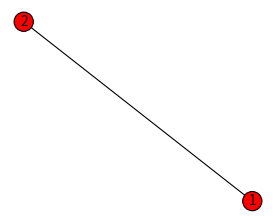
\includegraphics[scale=0.55]{line1.png}
\end{center}
% % % 네트워크에서 점의 위치와 엣지의 길이는 상관이 없다. 고려하지 않는다.
\end{frame}

\begin{frame}[fragile]
\frametitle{노드를 정의하는 방법}
\begin{block}{}
\begin{Verbatim}[numbers=left,commandchars=\\\{\}]
>>> G = nx.Graph()
>>> G.\textcolor{blue}{add_node}(`apple') \textcolor{red}{% 노드 `apple' 추가}
>>> G.\textcolor{blue}{add_nodes_from}([`banana',`kiwi',`mango']) 
\textcolor{red}{% 리스트로 추가 1}
or
>>> fruits = [`banana',`kiwi',`mango']
>>> G.add_nodes_from(fruits) \textcolor{red}{% 리스트로 추가 2}

>>> G.nodes() \textcolor{red}{% 노드들 보기}
[`apple', `kiwi', `mango', `banana']
\end{Verbatim}
\end{block}
\end{frame}

\begin{frame}[fragile]
\frametitle{엣지를 정의하는 방법}
\begin{block}{}
\begin{Verbatim}[numbers=left,commandchars=\\\{\}]
>>> G = nx.Graph()
>>> G.\textcolor{blue}{add_edge}(`apple', `banana') \tiny\textcolor{red}{% `apple'과 `banana'의 관계(엣지) 추가}
>>> G.\textcolor{blue}{add_edges_from}([(`apple',`mango'),(`apple',`kiwi')])
\textcolor{red}{% 리스트로 추가 1}
or
>>> relations = [(`apple',`mango'),(`apple',`kiwi')]
>>> G.add_edges_from(relations) \textcolor{red}{% 리스트로 추가 2}

>>> G.edges() \textcolor{red}{% 엣지들 보기}
[(`apple', `banana'), (`kiwi', `apple'), (`mango', `apple')]
\end{Verbatim}
\end{block}
\end{frame}

\begin{frame}[fragile]
\frametitle{노드의 속성 부여하기 1}
\begin{block}{}
\begin{Verbatim}[numbers=left,commandchars=\\\{\}]
>>> G.nodes()
[`kiwi', `mango', `apple', `banana']
>>> G.node[`kiwi']
\{\}
>>> G.node[`kiwi']{\textcolor{blue}{[`kind']}} = `fruit'
>>> G.node[`kiwi']
\{`kind': `fruit'\}
>>> G.nodes({\textcolor{red}{data=True}})
[(`kiwi', \{`kind': `fruit'\}), (`mango', \{\}), (`apple', \{\}),
 (`banana', \{\})]
\end{Verbatim}
\end{block}
\end{frame}

\begin{frame}[fragile]
\frametitle{노드의 속성 부여하기 2}
\begin{block}{}
\begin{Verbatim}[numbers=left,commandchars=\\\{\}]
>>> G.add_node(`kiwi', {\textcolor{blue}{kind=`fruit'}})
>>> G.add_nodes_from([`banana', `apple'], {\textcolor{blue}{kind=`fruit'}})
>>> G.node[`banana']
\{`kind': `fruit'\}
\end{Verbatim}
\end{block}
\end{frame}

\begin{frame}[fragile]
\frametitle{엣지에 속성 부여하기 1}
\begin{block}{}
\begin{Verbatim}[numbers=left,commandchars=\\\{\}]
>>> G.edges()
[(`kiwi', `apple'), (`mango', `apple'), (`apple', `banana')]
>>> G.edges({\textcolor{red}{data=True}})
[(`kiwi', `apple', \{\}), (`mango', `apple', \{\}), (`apple',
 `banana', \{\})]
 
>>> G.add_edge(`apple', `mango', {\textcolor{blue}{weight=2.5}})
>>> G.add_edges_from(relations, {\textcolor{blue}{color=`blue'}})
>>> G[`apple'][`mango']{\textcolor{blue}{[`weight']}}=5
>>> G.edge[`apple'][`kiwi']{\textcolor{blue}{[`weight']}}=2
\end{Verbatim}
\end{block}
\end{frame}

\begin{frame}[fragile]
\frametitle{엣지에 속성 부여하기 2}
\begin{block}{}
\begin{Verbatim}[numbers=left,commandchars=\\\{\}]
>>> G.edges({\textcolor{blue}{data=True}})
[(`kiwi', `apple', \{`color': `blue'\}),
 (`mango', `apple', \{`color': `blue', `weight': 5\}),
 (`apple', `banana', \{\})]
\end{Verbatim}
\end{block}
\end{frame}

%------------------------------------------------

\section{네트워크 그리기}

\begin{frame}
\frametitle{네트워크 그리기}
\textbf{네트워크가 정의되기 위해서는?}
\begin{itemize}
\item 점(Objects, Vertices, Nodes, Sites, Actors, ...)
\item 선(Relations, Edges, Links, Bonds, Ties, ...)
\end{itemize}
{\hspace{8mm}\textbf{$+$}}
\begin{itemize}
\item 점의 위치
\end{itemize}
\end{frame}

\begin{frame}[fragile]
\frametitle{네트워크 그리기}
\begin{block}{}
\begin{Verbatim}[numbers=left,commandchars=\\\{\}]
>>> G = nx.Graph()
>>> relations = [(`apple', `banana'), (`kiwi', `apple'), 
(`mango', `apple')]
>>> G.add_edges_from(relations) \textcolor{red}{% 점, 선 생성}
>>> \color{blue}{nx.draw(G)} \textcolor{red}{% 점의 위치를 spring layout으로 생성}
>>> plt.show()
\end{Verbatim}
\end{block}
\begin{center}
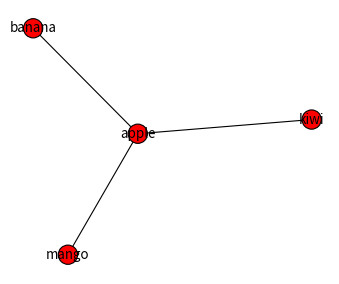
\includegraphics[scale=0.55]{network_basic1.jpg}
\end{center}
\end{frame}

\begin{frame}[fragile]
\frametitle{네트워크 그리기}
\begin{block}{}
\begin{Verbatim}[numbers=left,commandchars=\\\{\}]
>>> nx.{\color{magenta}{draw}}(G) \color{gray}{% 기본 그리기}
>>> nx.draw_{\color{blue}{circular}}(G) \color{gray}{% 원 위에 노드 놓기}
>>> nx.draw_{\color{blue}{graphviz}}(G) \color{gray}{% Graphviz 사용}
>>> nx.draw_{\color{blue}{random}}(G) \color{gray}{% 균등 분포를 이용한 랜덤}
>>> nx.draw_{\color{blue}{shell}}(G) \color{gray}{% 동심원 위에 노드 놓기}
>>> nx.draw_{\color{blue}{spectral}}(G) \color{gray}{% 그래프 라플라시안의 고유 벡터 기반}
>>> nx.draw_{\color{blue}{spring}}(G)\tiny \color{gray}{% Fruchterman-Reingold force-directed alg. 기반}
\end{Verbatim}
\end{block}
\end{frame}

\begin{frame}[fragile]
\frametitle{점의 위치 정하기}
\begin{block}{}
\begin{Verbatim}[numbers=left,commandchars=\\\{\}]
>>> {\color{red}{pos}} = nx.{\color{blue}{spectral}}_layout(G) \color{gray}{% nx.spring_layout, ...}
>>> print pos
\{'kiwi': array([ 1.,  0.]), 'mango': array([ 0.,  1.]), 
'apple': array([ 0.66666667,  0.66666667]), 'banana':
 array([ 1.,  1.])\}
 
>>> nx.draw(G, {\color{red}{pos}})
>>> plt.show()
\end{Verbatim}
\end{block}
\end{frame}

\begin{frame}
\frametitle{지금까지 한 것}
\textbf{지금까지 한 것}
\begin{itemize}
\item 점, 선 정의
\item 점, 선 속성 정의
\item 점 위치 정의
\end{itemize}
{\color{white}
\textbf{뒤에서 할 것}
\begin{itemize}
\item \color{white}점의 특징 계산
\end{itemize}
}
\end{frame}

\begin{frame}
\frametitle{지금까지 한 것}
\textbf{지금까지 한 것}
\begin{itemize}
\item 점, 선 정의
\item 점, 선 속성 정의
\item 점 위치 정의
\end{itemize}
\textbf{뒤에서 할 것}
\begin{itemize}
\item 점의 {\textcolor{red}{특징}} 계산
\end{itemize}
\end{frame}
% 여기에 하나 더 점의 특징을 계산하는 것을 해볼 것입니다. 점의 특징을 계산한다는 건 어떤 걸까요?

%------------------------------------------------
\section{네트워크 계산}

\begin{frame}[fragile]
\frametitle{네트워크 계산}
\begin{block}{각 점의 특징 계산}
\begin{Verbatim}[numbers=left,commandchars=\\\{\}]
>>> G.nodes()
[`kiwi', `mango', `apple', `banana']
>>> nx.to_numpy_matrix(G)
matrix([[ 0.,  0.,  1.,  0.],
        [ 0.,  0.,  1.,  0.],
        [ 1.,  1.,  0.,  1.],
        [ 0.,  0.,  1.,  0.]])
\end{Verbatim}
\end{block}
\begin{center}
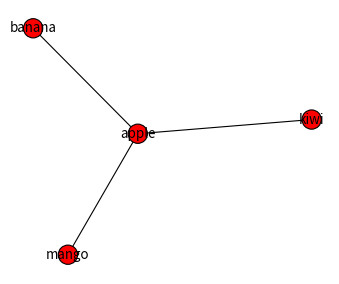
\includegraphics[scale=0.35]{network_basic1.jpg}
\end{center}
\end{frame}

\begin{frame}[fragile]
\frametitle{네트워크 $\Rightarrow$ 행렬 $\Rightarrow$ ?$_1$}
\begin{center}
\huge
\(
  \begin{bmatrix}
    0 & 0 & 1 & 0\\
    0 & 0 & 1 & 0\\
    1 & 1 & 0 & 1\\
    0 & 0 & 1 & 0\\
  \end{bmatrix}
\)
\end{center}
\end{frame}

\begin{frame}[fragile]
\frametitle{네트워크 $\Rightarrow$ 행렬 $\Rightarrow$ ?$_1$}
\begin{center}
\huge
\(
  \begin{bmatrix}
    0 & 0 & 1 & 0\\
    0 & 0 & 1 & 0\\
    1 & 1 & 0 & 1\\
    0 & 0 & 1 & 0\\
  \end{bmatrix}
\)
=
\(
  \begin{bmatrix}
    1\\
    1\\
    3\\
    1\\
  \end{bmatrix}
\)
\end{center}
\end{frame}

\begin{frame}[fragile]
\frametitle{Degree 계산하기}
\begin{block}{}
	\begin{Verbatim}[numbers=left,commandchars=\\\{\}]
	>>> print G.degree()
	{`kiwi': 1, `mango': 1, `apple': 3, `banana': 1}
	\end{Verbatim}
\end{block}
\begin{center}
\(
  \begin{bmatrix}
    0 & 0 & 1 & 0\\
    0 & 0 & 1 & 0\\
    1 & 1 & 0 & 1\\
    0 & 0 & 1 & 0\\
  \end{bmatrix}
\)
=
\(
  \begin{bmatrix}
    1\\
    1\\
    3\\
    1\\
  \end{bmatrix}
\)
\end{center}
\end{frame}

\begin{frame}[fragile]
\frametitle{Degree에 따른 노드의 크기 변화}
\begin{block}{}
	\begin{Verbatim}[numbers=left,commandchars=\\\{\}]
>>> relations = [(`kiwi', `apple'), (`mango', `apple'),
(`apple', `banana')]
>>> G.add_edges_from(relations)
>>> degree = nx.degree(G)
>>> nx.draw(G, {\textcolor{blue}{node_size=[v*1000 for v in degree.values()]}})
>>> plt.show()
	\end{Verbatim}
\end{block}
\begin{center}
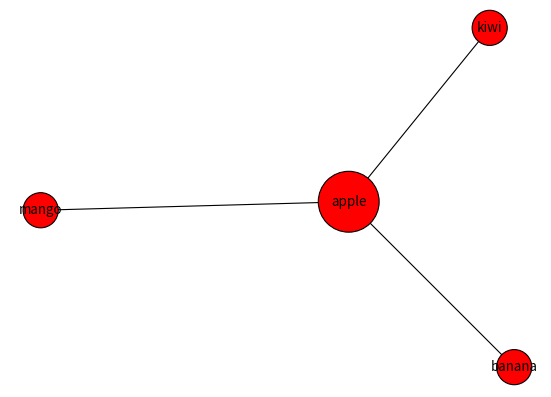
\includegraphics[scale=0.35]{nodesize.png}
\end{center}
\end{frame}

\begin{frame}[fragile]
\frametitle{nx.draw()}
\begin{block}{}
	\begin{Verbatim}[numbers=left,commandchars=\\\{\}]
nx.draw(G, pos=None, ax=None, hold=None, {\textcolor{red}{**kwds}})
\textcolor{red}{\href{https://networkx.github.io/documentation/latest/reference/generated/networkx.drawing.nx_pylab.draw_networkx.html#networkx.drawing.nx_pylab.draw_networkx}{kwds 문서 링크}}
: pos, with_labels, ax, nodelist, edgelist, node_size,
 node_color, node_shape, alpha, cmap, vmin, vmax,
 linewidths, width, edge_color, edge_cmap, edge_vmin,
 edge_vmax, style, labels, font_size, font_color,
 font_weight, font_family, label, ...
	\end{Verbatim}
\end{block}
\end{frame}
% kwds optional keywords가 붙어 있습니다.

{
\fbckg{degree_distribution.png}
\begin{frame}[fragile]
\frametitle{Degree Rank 그리기}
\tiny\begin{Verbatim}[numbers=left,commandchars=\\\{\}]
__author__ = """Aric Hagberg <aric.hagberg@gmail.com>""" {\textcolor{red}{\href{http://networkx.github.io/documentation/latest/examples/drawing/degree_histogram.html}{문서 링크}}}
import networkx as nx
import matplotlib.pyplot as plt
G = nx.{\textcolor{blue}{gnp_random_graph(100,0.02)}} % binomial_graph 생성

degree_sequence=sorted({\textcolor{blue}{nx.degree(G).values()}},reverse=True) # Degree 리스트 값 생성
dmax=max(degree_sequence)

plt.loglog(degree_sequence,'b-',marker='o')
plt.title("Degree rank plot")
plt.ylabel("degree")
plt.xlabel("rank")

# draw graph in inset
plt.axes([0.45,0.45,0.45,0.45])
pos=nx.spring_layout(G)
plt.axis('off')
nx.draw_networkx_nodes(G,pos,node_size=20)
nx.draw_networkx_edges(G,pos,alpha=0.4)

plt.savefig("degree_rank.png")
\end{Verbatim}
\end{frame}
}

{
\fbckg{degree_distribution2.png}
\begin{frame}[fragile]
\frametitle{Degree 분포 그리기}
\tiny\begin{Verbatim}[numbers=left,commandchars=\\\{\}]
__author__ = """Aric Hagberg <aric.hagberg@gmail.com>"""
import networkx as nx
import matplotlib.pyplot as plt
G = nx.{\textcolor{blue}{gnp_random_graph(100,0.02)}} # binomial_graph 생성

degrees = nx.degree(G).values()
dmax=max(degrees)

h, bins = np.histogram(degrees, bins=dmax)
hmax = max(h)
plt.axis([1, dmax, 1, hmax])
x=bins.compress(h)
y=h.compress(h)

plt.loglog(x,y, 'bo-')
plt.title("Degree distribution")
plt.xlabel("degree")
plt.ylabel("number of nodes")
plt.savefig("degree_distribution.png")
plt.show()
# plt.axes([0.1,0.1,0.5,0.5])
\end{Verbatim}
\end{frame}
}

\begin{frame}[fragile]
\frametitle{네트워크 $\Rightarrow$ 행렬 $\Rightarrow$ ?$_2$}
\begin{center}
\huge
{\(
  \begin{bmatrix}
    0 & 0 & 1 & 0\\
    0 & 0 & 1 & 0\\
    1 & 1 & 0 & 1\\
    0 & 0 & 1 & 0\\
  \end{bmatrix}
\)$^2$}
=
\(
  \begin{bmatrix}
    1 & 1 & 0 & 1\\
    1 & 1 & 0 & 1\\
    0 & 0 & 3 & 0\\
    1 & 1 & 0 & 1\\
  \end{bmatrix}
\)
\end{center}
\end{frame}

\begin{frame}[fragile]
\frametitle{네트워크 $\Rightarrow$ 행렬 $\Rightarrow$ ?$_2$}
\begin{center}
\large
{\(
  \begin{bmatrix}
    0 & 0 & 1 & 0\\
    0 & 0 & 1 & 0\\
    1 & 1 & 0 & 1\\
    0 & 0 & 1 & 0\\
  \end{bmatrix}
\)$^2$}
=
\(
  \begin{bmatrix}
    1 & 1 & 0 & 1\\
    1 & 1 & 0 & 1\\
    0 & 0 & 3 & 0\\
    1 & 1 & 0 & 1\\
  \end{bmatrix}
\)
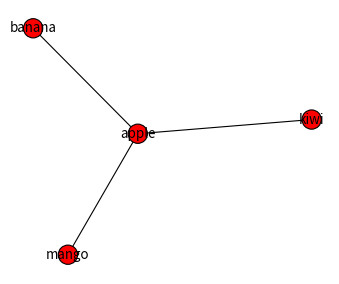
\includegraphics[scale=0.7]{network_basic1.jpg}
\end{center}
\begin{Verbatim}[numbers=left,commandchars=\\\{\}]
>>> G.nodes()
[`kiwi', `mango', `apple', `banana']
\end{Verbatim}
\end{frame}

\begin{frame}[fragile]
\frametitle{네트워크 $\Rightarrow$ 행렬 $\Rightarrow$ ?$_2$}
\begin{block}{}
	\begin{Verbatim}[numbers=left,commandchars=\\\{\}]
>>> A = nx.to_numpy_matrix(G)
>>> print A
matrix([[ 0.,  0.,  1.,  0.],
        [ 0.,  0.,  1.,  0.],
        [ 1.,  1.,  0.,  1.],
        [ 0.,  0.,  1.,  0.]])
>>> print A**2
matrix([[ 1.,  1.,  0.,  1.],
        [ 1.,  1.,  0.,  1.],
        [ 0.,  0.,  3.,  0.],
        [ 1.,  1.,  0.,  1.]])
	\end{Verbatim}
\end{block}
\end{frame}

\begin{frame}[fragile]
\frametitle{경로 길이}
\begin{center}
\huge
{\(
  \begin{bmatrix}
    0 & 0 & 1 & 0\\
    0 & 0 & 1 & 0\\
    1 & 1 & 0 & 1\\
    0 & 0 & 1 & 0\\
  \end{bmatrix}
\)$^2$}
=
\(
  \begin{bmatrix}
    1 & 1 & 0 & 1\\
    1 & 1 & 0 & 1\\
    0 & 0 & 3 & 0\\
    1 & 1 & 0 & 1\\
  \end{bmatrix}
\)
\end{center}
\begin{equation*}
N_{ij}^{(2)}=\sum_{k=1}^{n}A_{ik}A_{kj}=[\mathbf{A}^2]_{ij}
\end{equation*}
\begin{equation*}
N_{ij}^{(3)}=\sum_{k,l=1}A_{ik}A_{kl}A_{lj}=[\mathbf{A}^3]_{ij}
\end{equation*}
\end{frame}

\begin{frame}
\frametitle{최단 경로}
\textbf{최단 경로 알고리즘} {\tiny{\textcolor{red}{\href{http://networkx.lanl.gov/reference/generated/networkx.algorithms.shortest_paths.generic.shortest_path.html}{문서 링크}}}}
\begin{itemize}
\item nx.shortest\_path
\item nx.all\_shortest\_paths
\item nx.shortest\_path\_length
\item nx.average\_shortest\_path\_length
\item nx.has\_path
\end{itemize}
\textbf{다익스트라 알고리즘}
\begin{itemize}
\item dijkstra\_path
\item dijkstra\_path\_length
\end{itemize}
\end{frame}

\begin{frame}[fragile]
\frametitle{네트워크의 중심성}
\begin{block}{}
	\begin{Verbatim}[numbers=left,commandchars=\\\{\}]
>>> nx.betweenness_centrality(G)
{`kiwi': 0.0, `mango': 0.0, `apple': 1.0, `banana': 0.0}
>>> nx.closeness_centrality(G)
{`kiwi': 0.6, `mango': 0.6, `apple': 1.0, `banana': 0.6}
>>> nx.degree_centrality(G)
{`kiwi': 0.33, `mango': 0.33, `apple': 1.0, `banana': 0.33}
	\end{Verbatim}
\end{block}
\textcolor{red}{\href{http://www.slideshare.net/koorukuroo/network-analysis-with-networkx-fundamentals-of-network-theory1}{내용 설명 링크}} {\tiny{71페이지, 66페이지, 60페이지}}
\end{frame}

\begin{frame}[fragile]
\frametitle{네트워크 $\Rightarrow$ 행렬 $\Rightarrow$ ?$_3$}
\begin{center}
\huge
\(
  \begin{bmatrix}
    0 & 0 & 1 & 0\\
    0 & 0 & 1 & 0\\
    1 & 1 & 0 & 1\\
    0 & 0 & 1 & 0\\
  \end{bmatrix}
\)
\end{center}
\end{frame}

\begin{frame}[fragile]
\frametitle{행렬의 고유값, 고유벡터}
\begin{block}{}
\small
	\begin{Verbatim}[numbers=left,commandchars=\\\{\}]
>>> A = nx.to_numpy_matrix(G)
>>> [w,v]=np.linalg.eig(A)
>>> w # eigenvalues
array([ -1.73205081e+00,   1.79977561e-17,   1.73205081e+00,
         0.00000000e+00])
>>> v # normalized eigenvectors
matrix([[  4.08248290e-01,  -8.16496581e-01,   4.08248290e-01,
           0.00000000e+00],
        [  4.08248290e-01,   4.08248290e-01,   4.08248290e-01,
          -7.07106781e-01],
        [ -7.07106781e-01,   9.45046688e-17,   7.07106781e-01,
           0.00000000e+00],
        [  4.08248290e-01,   4.08248290e-01,   4.08248290e-01,
           7.07106781e-01]])
	\end{Verbatim}
\end{block}
\end{frame}

\begin{frame}[fragile]
\frametitle{고유벡터 중심성}
\begin{block}{}
	\begin{Verbatim}[numbers=left,commandchars=\\\{\}]
>>> nx.{\textcolor{blue}{eigenvector_centrality}}(G)
Traceback (most recent call last)
  File <stdin>, line 1, in <module>
    File eigenvector.py, line 103, in eigenvector_centrality
      power iteration failed to converge in %d iterations.
  networkx.exception.NetworkXError eigenvector_centrality(): 
  power iteration failed to converge in %d iterations.%(i+1)
	\end{Verbatim}
\end{block}
\textcolor{red}{\href{http://www.slideshare.net/koorukuroo/network2-35160056}{내용 설명 링크}} {\tiny{58페이지}}
\end{frame}

\begin{frame}[fragile]
\frametitle{NetworkX 내용 정리}
\begin{itemize}
\item 데이터 추상화
\item 객체(노드)와 관계(엣지)의 자유로운 정의
\item import networkx as nx
\item G = nx.Graph()
\item 노드, 엣지 추가
\item 노드, 엣지 속성 부여
\item 네트워크 그리기
\item 행렬 아이디어 ?$_1$, ?$_2$, ?$_3$
\end{itemize}
\end{frame}

%------------------------------------------------
\section{데모}
\begin{frame}
\frametitle{데모}
\begin{enumerate}
\item 드라마 네트워크
\item 프로그래밍 언어 네트워크
\item 페이스북 네트워크
\end{enumerate}
\end{frame}

\subsection{드라마 네트워크}
\begin{frame}[fragile]
\frametitle{드라마 대본을 이용한 네트워크}
\begin{block}{}
	\begin{Verbatim}[numbers=left,commandchars=\\\{\}]
부산과학고등학교 2014 R&E
연구자 : 권기영, 김채린, 배지환, 이가영, 한송미
	\end{Verbatim}
\end{block}
\begin{center}

\includegraphics[scale=0.5]{couple.png}
\end{center}
\end{frame}

\begin{frame}
\frametitle{드라마 대본을 이용한 네트워크}
한국콘텐츠진흥원 KOCCA 방송대본데이터베이스\\
\href{http://db.kocca.kr/db/bbs/read/broadcastdb.do?nttNo=1931073}{http://db.kocca.kr/db/bbs/read/broadcastdb.do?nttNo=1931073}
\begin{center}
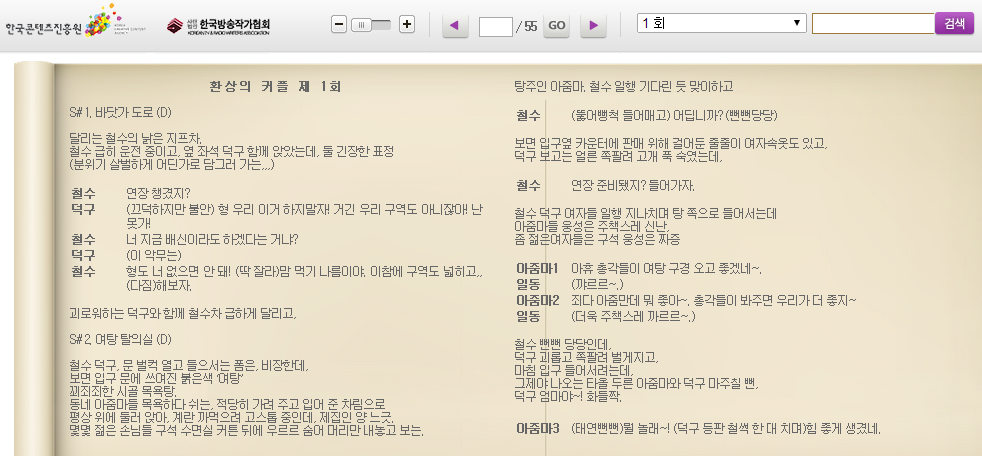
\includegraphics[scale=0.5]{kocca.png}
\end{center}
\end{frame}

\begin{frame}[fragile]
\frametitle{드라마 대본을 이용한 네트워크}
\textbf{동시 출현성 (Co-Occurrence)}
\begin{itemize}
\item 객체(노드) : 등장인물\\
\item 관계(엣지) : 같은 문장 내에 등장하는 인물들
\end{itemize}
\begin{block}{}
\scriptsize
	\begin{Verbatim}[numbers=left,commandchars=\\\{\}]
그래. 아깐 정말 폭풍전야 같았어. 장철수는 이제 안나한테 죽~었어~!!
	\end{Verbatim}
\end{block}
\begin{center}
장철수 - 안나
\end{center}
\end{frame}

\begin{frame}[fragile]
\frametitle{드라마 대본을 이용한 네트워크}
\textbf{동시 출현성 (Co-Occurrence)}
\begin{itemize}
\item 객체(노드) : 등장인물\\
\item 관계(엣지) : 화자(말하는 사람)가 언급하는 인물
\end{itemize}
\begin{block}{}
\scriptsize
	\begin{Verbatim}[numbers=left,commandchars=\\\{\}]
\textbf{빌리}	:	그래. 아깐 정말 폭풍전야 같았어. 장철수는 이제 안나한테 죽~었어~!!
	\end{Verbatim}
\end{block}
\begin{center}
빌리 - 장철수\\
빌리 - 안나
\end{center}
\end{frame}

\begin{frame}[fragile]
\frametitle{드라마 대본을 이용한 네트워크}
\huge
\begin{center}
노드({\color{blue}{Node}})와 엣지({\color{red}{Edge}})는\\
어떤 것도 될 수 있다!
\end{center}
\end{frame}

\begin{frame}[fragile]
\frametitle{드라마 대본을 이용한 네트워크}
\begin{block}{}
\scriptsize
	\begin{Verbatim}[numbers=left,commandchars=\\\{\}]
{\color{blue}{\textbf{씬/45 철수집 거실 (D)}}}
철수 화장실 나와서
 ‘전화가 왜 이렇게 돼 있냐,,’ 툭 올려 두고, ‘근데 내 핸드폰 어딨냐,,’ 찾는데
안나 핸드폰 꽂아 둔 쇼파위에 깔고 앉는다.

\textbf{안나}	:	꼬시다 꽃다발.. (썩소 하는데)
\textbf{철수}	:	(나두고 가지뭐,,) 나 나간다. 애들 밥 챙겨라. (하고)
\textbf{안나}	:	에씨.. 왜 또 기어나가는 거야. 지금 가면 꽃다발 만날 텐데..

{\color{blue}{\textbf{씬/46 철수마당 (D)}}}
철수 나가는데 안나 나오며 ‘장철수~’
철수 보면

\textbf{안나}	:	꽃순이 집이 부서진 거 같던데, 봤어? 고쳐 주고 가.
\textbf{철수}	:	꽃순이가 일부러 부서논 거야. (가면)
	\end{Verbatim}
\end{block}
\end{frame}

\begin{frame}[fragile]
\frametitle{드라마 대본을 이용한 네트워크}
\textbf{동시 출현성 (Co-Occurrence)}
\begin{itemize}
\item 객체(노드) : 등장인물\\
\item 관계(엣지) : 같은 씬에 등장하는 인물들
\end{itemize}
\begin{block}{}
\scriptsize
\begin{Verbatim}[numbers=left,commandchars=\\\{\}]
s = read(filename)
contents = s.{\color{red}{split}}(`씬/')
for content in contents:
\hspace{6mm}...
\hspace{6mm}G.add_edge(등장인물1, 등장인물2)
\hspace{6mm}...

\end{Verbatim}
\end{block}
\end{frame}

{
\fbckg{couple_network1.png}
\begin{frame}[fragile]
\frametitle{드라마 대본을 이용한 네트워크}
\scriptsize
\begin{Verbatim}[numbers=left,commandchars=\\\{\}]
\hspace{15mm}degree = nx.degree(G).values()
\hspace{15mm}nx.draw(G, node_size=[v*1000 for v in degree], font_size=30)
\hspace{15mm}plt.show()
\end{Verbatim}
\vspace{7cm}
%\begin{center}
%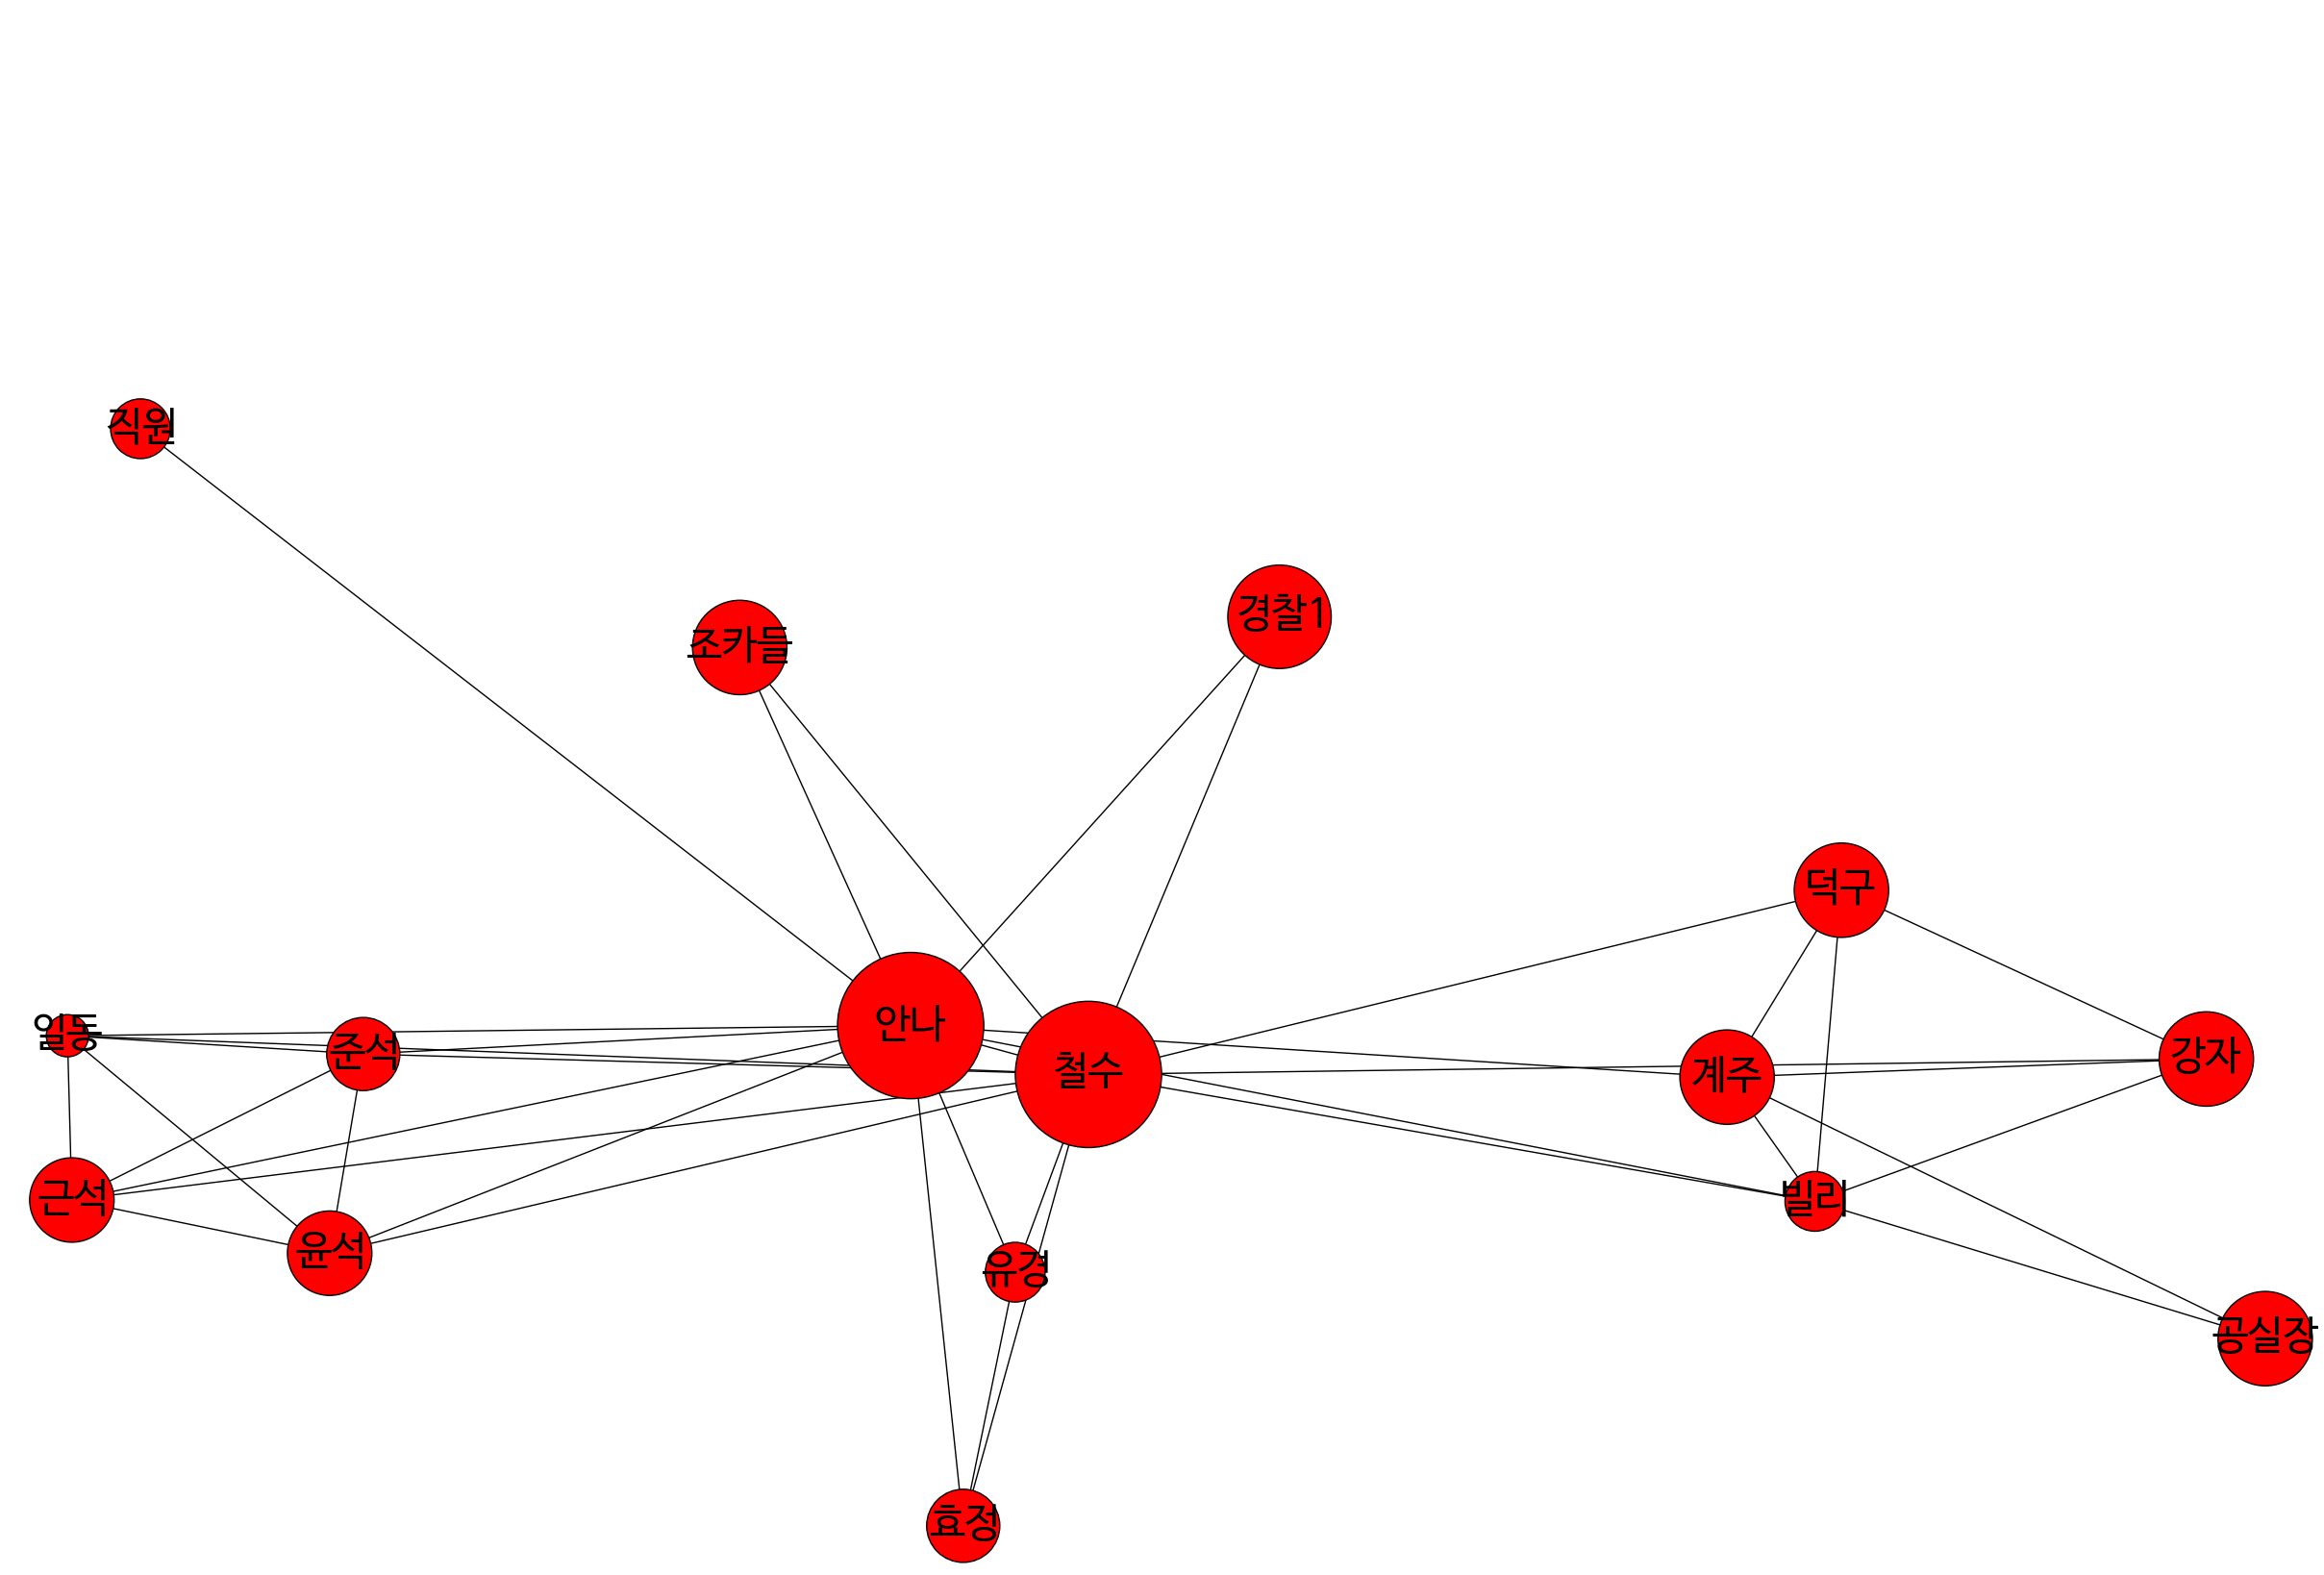
\includegraphics[scale=0.2]{couple_network1.png}
%\end{center}
\end{frame}
}

\begin{frame}[fragile]
\frametitle{드라마 대본을 이용한 네트워크}
\textbf{Network Information}
\scriptsize
\begin{block}{}
\begin{Verbatim}[numbers=left,commandchars=\\\{\}]
    print "Number of Nodes : ", nx.number_of_nodes(G)
    print "Number of Edges : ", nx.number_of_edges(G)
    degreelist = list(G.degree().values())
    print "Avg. Node Degree : ", float(sum(degreelist))/nx.number_of_nodes(G)
    print "Avg. Path Length : ", nx.average_shortest_path_length(G)
    print "Avg. Clustering Coefficient : ", nx.average_clustering(G)
\end{Verbatim}
\end{block}
\begin{Verbatim}[numbers=left,commandchars=\\\{\}]
Number of Nodes :  16
Number of Edges :  38
Avg. Node Degree :  4.75
Avg. Path Length :  1.775
Avg. Clustering Coefficient :  0.765340909091
\end{Verbatim}
\end{frame}

\begin{frame}[fragile]
\frametitle{드라마 대본을 이용한 네트워크}
\textbf{Network Information}
\scriptsize
\begin{block}{}
\begin{Verbatim}[numbers=left,commandchars=\\\{\}]
    print "::: Betweenness Centrality"
    x = nx.betweenness_centrality(G)
    sorted_list = sorted(x.iteritems(), key=operator.itemgetter(1), reverse=True)
    for s in sorted_list[:20]:
        print s[0], s[1]
\end{Verbatim}
\end{block}
\begin{Verbatim}[numbers=left,commandchars=\\\{\}]
::: Betweenness Centrality
안나 0.400793650794
철수 0.328571428571
빌리 0.0944444444444
계주 0.0571428571429
강자 0.00238095238095
덕구 0.00238095238095
\end{Verbatim}
\end{frame}

\begin{frame}[fragile]
\frametitle{드라마 대본을 이용한 네트워크}
\textbf{Network Information}
\scriptsize
\begin{block}{}
\begin{Verbatim}[numbers=left,commandchars=\\\{\}]
    print "::: Closeness Centrality"
    x = nx.closeness_centrality(G)
    sorted_list = sorted(x.iteritems(), key=operator.itemgetter(1), reverse=True)
    for s in sorted_list[:20]:
        print s[0], s[1]
\end{Verbatim}
\end{block}
\begin{Verbatim}[numbers=left,commandchars=\\\{\}]
::: Closeness Centrality
안나 0.833333333333
철수 0.833333333333
빌리 0.625
계주 0.6
근석 0.576923076923
일동 0.576923076923
\end{Verbatim}
\end{frame}

\begin{frame}[fragile]
\frametitle{드라마 대본을 이용한 네트워크}
\textbf{참고자료}
\begin{itemize}
\item {\color{blue}{\href{http://www.hscoaching.com/301}{언어 네트워크 분석으로 신뢰-비신뢰 요인 한눈에 본다}}}
\item {\color{blue}{\href{http://www.kipa.re.kr/public/institute/institute_view.jsp?c=&pagenum=4&seqno=933&boardid=40&typeID=50&tableName=TB_TEST02}{공공앱의 사용자 리뷰에 대한 분석 : 언어네트워크분석을 중심으로}}}
\end{itemize}
\end{frame}

\begin{frame}[fragile]
\frametitle{드라마 대본을 이용한 네트워크}
\textbf{참고자료}
\begin{itemize}
\item \href{http://www.hscoaching.com/301}{언어 네트워크 분석으로 신뢰-비신뢰 요인 한눈에 본다}
\end{itemize}
\begin{center}
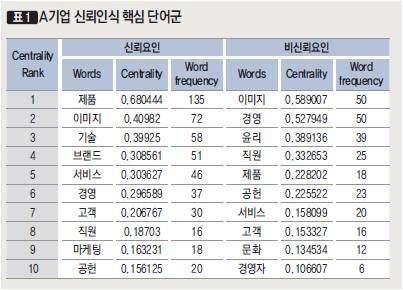
\includegraphics[scale=0.8]{hscoaching_1.jpg}
\end{center}
\end{frame}

\begin{frame}[fragile]
\frametitle{드라마 대본을 이용한 네트워크}
\textbf{참고자료}
\begin{itemize}
\item \href{http://www.hscoaching.com/301}{언어 네트워크 분석으로 신뢰-비신뢰 요인 한눈에 본다}
\end{itemize}
\begin{center}
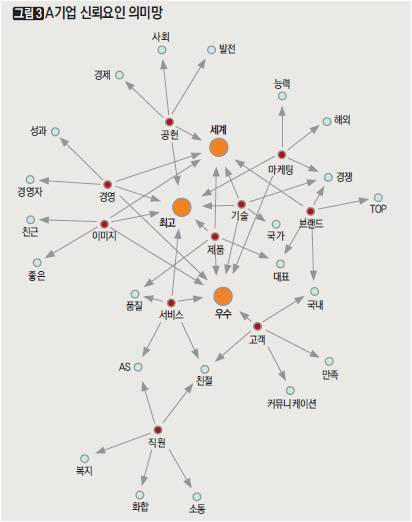
\includegraphics[scale=0.4]{hscoaching_2.jpg}
\end{center}
\end{frame}

\begin{frame}[fragile]
\frametitle{드라마 대본을 이용한 네트워크}
\textbf{참고자료}
\begin{itemize}
\item \href{http://www.kipa.re.kr/public/institute/institute_view.jsp?c=&pagenum=4&seqno=933&boardid=40&typeID=50&tableName=TB_TEST02}{공공앱의 사용자 리뷰에 대한 분석 : 언어네트워크분석을 중심으로}
\end{itemize}
\begin{center}
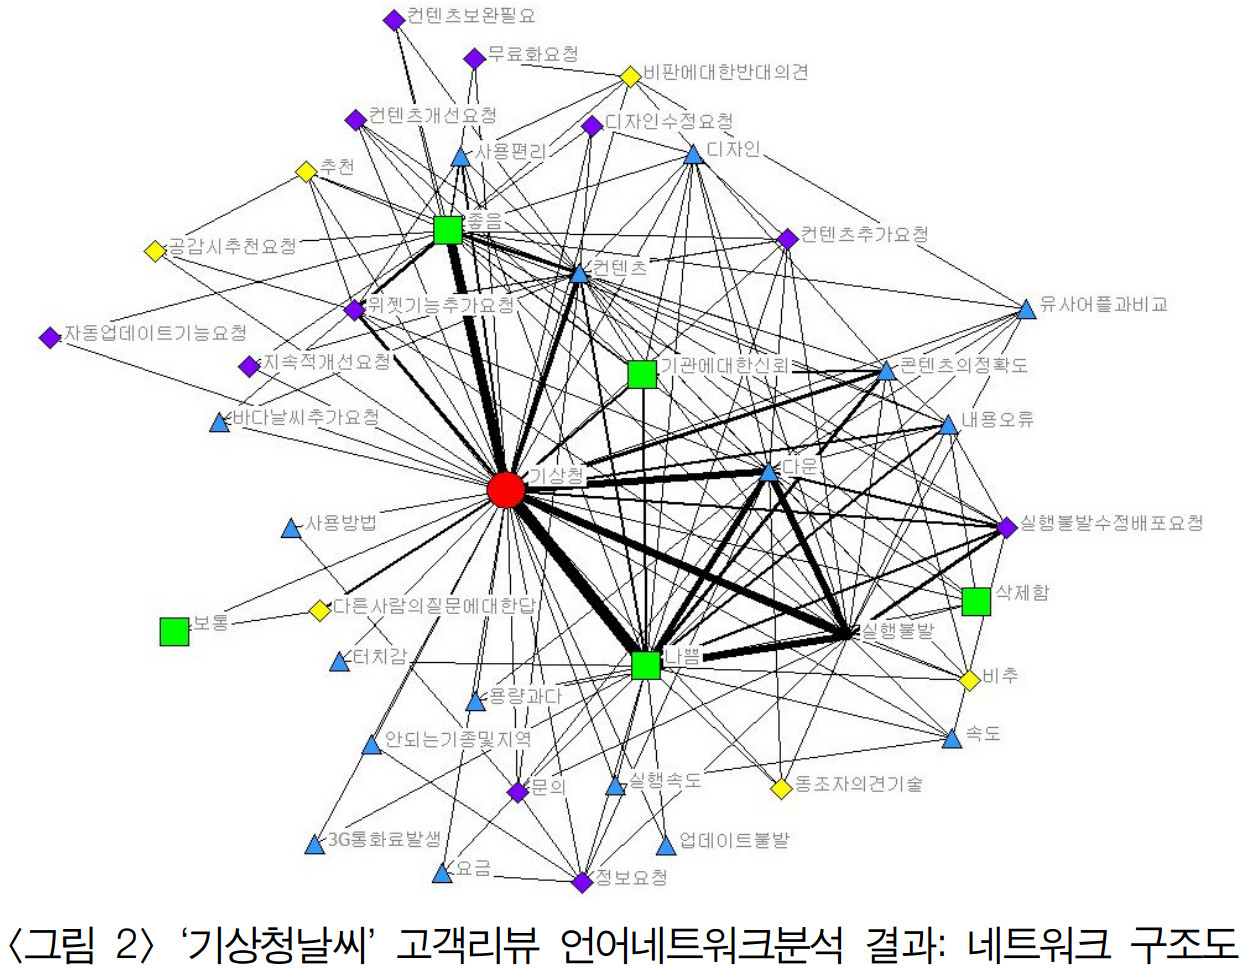
\includegraphics[scale=0.3]{weather.jpg}
\end{center}
\end{frame}


\begin{frame}
\frametitle{드라마 대본을 이용한 네트워크}
\textbf{한국어 대사 분석 방법}
\begin{center}

\includegraphics[scale=0.6]{nlp.png}
\end{center}
\end{frame}

\subsection{프로그래밍 언어 네트워크}

{
\fbckg{language_degree.png}
\begin{frame}[fragile]
\frametitle{프로그래밍 언어 네트워크}
\tiny
\begin{Verbatim}[numbers=left,commandchars=\\\{\}]
{\large{Document :}}
\href{http://brendangriffen.com/gow-programming-languages/}{http://brendangriffen.com/gow-programming-languages/}

{\large{Python :}}
\href{https://github.com/bgriffen/griffsgraphs/blob/master/programminglanguages/proglanguages.py}{https://github.com/bgriffen/griffsgraphs/blob/master/programminglanguages/proglanguages.py}

{\large{Dataset :}} 
\href{https://github.com/bgriffen/griffsgraphs/tree/master/programminglanguages/data/languages}{https://github.com/bgriffen/griffsgraphs/tree/master/programminglanguages/data/languages}
\end{Verbatim}
\end{frame}
}

\begin{frame}
\frametitle{프로그래밍 언어 네트워크}
\begin{center}
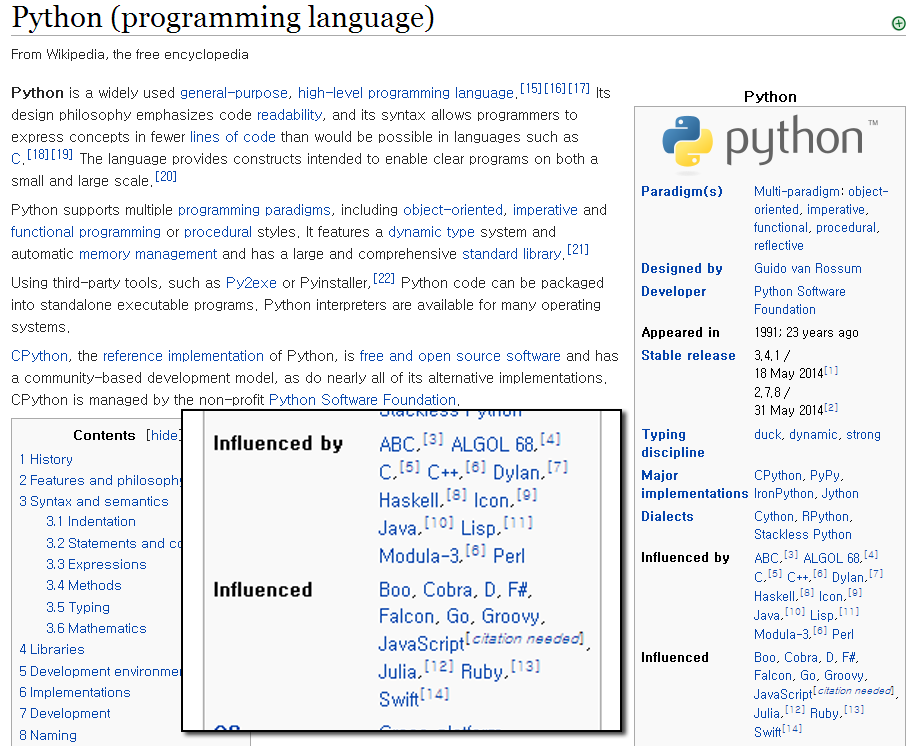
\includegraphics[scale=0.45]{python.png}
\end{center}
\end{frame}

{
\fbckg{language_degree2.png}
\begin{frame}
\frametitle{프로그래밍 언어 네트워크}
\tiny
\color{blue}{Node Size = Degree}
\end{frame}
}

{
\fbckg{language_pagerank.png}
\begin{frame}
\frametitle{프로그래밍 언어 네트워크}
\tiny
\color{blue}{Node Size = \href{http://www.slideshare.net/koorukuroo/network2-35160056}{PageRank}}
\end{frame}
}

\begin{frame}
\frametitle{프로그래밍 언어 네트워크}
\textbf{웹 크롤링 방법}
\begin{center}

\includegraphics[scale=0.6]{scrapper.png}
\end{center}
\end{frame}


\subsection{페이스북 친구 네트워크}
\begin{frame}
\frametitle{페이스북 친구 네트워크}
\textbf{Netvizz}
\begin{center}

\includegraphics{netvizz_1.png}
\end{center}
\end{frame}

\begin{frame}
\frametitle{페이스북 친구 네트워크}
\textbf{Netvizz}
\begin{center}
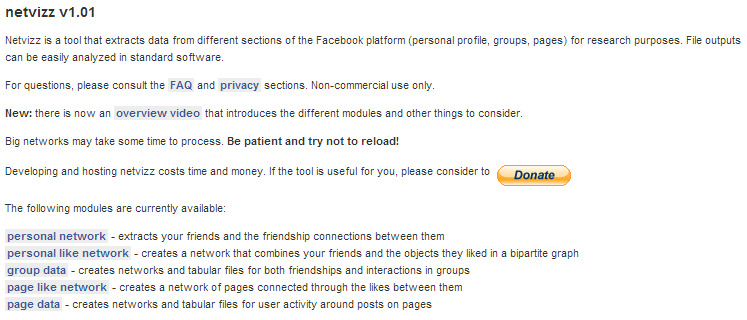
\includegraphics[scale=0.9]{netvizz_2.png}
\end{center}
\end{frame}

\begin{frame}
\frametitle{페이스북 친구 네트워크}
\textbf{Netvizz}
\begin{center}
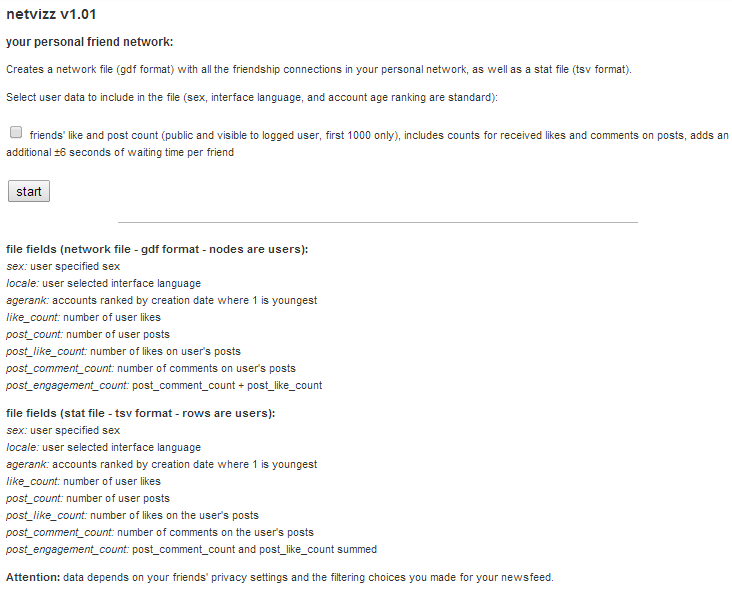
\includegraphics[scale=0.7]{netvizz_3.png}
\end{center}
\end{frame}

\begin{frame}
\frametitle{페이스북 친구 네트워크}
\textbf{Netvizz}
\begin{center}
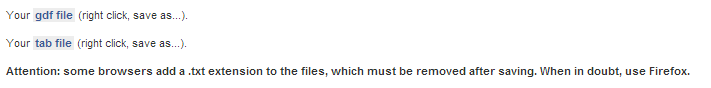
\includegraphics[scale=0.7]{netvizz_4.png}
\end{center}
\end{frame}

\begin{frame}
\frametitle{페이스북 친구 네트워크}
\textbf{페이스북 네트워크 with Degree Centrality}
\begin{center}
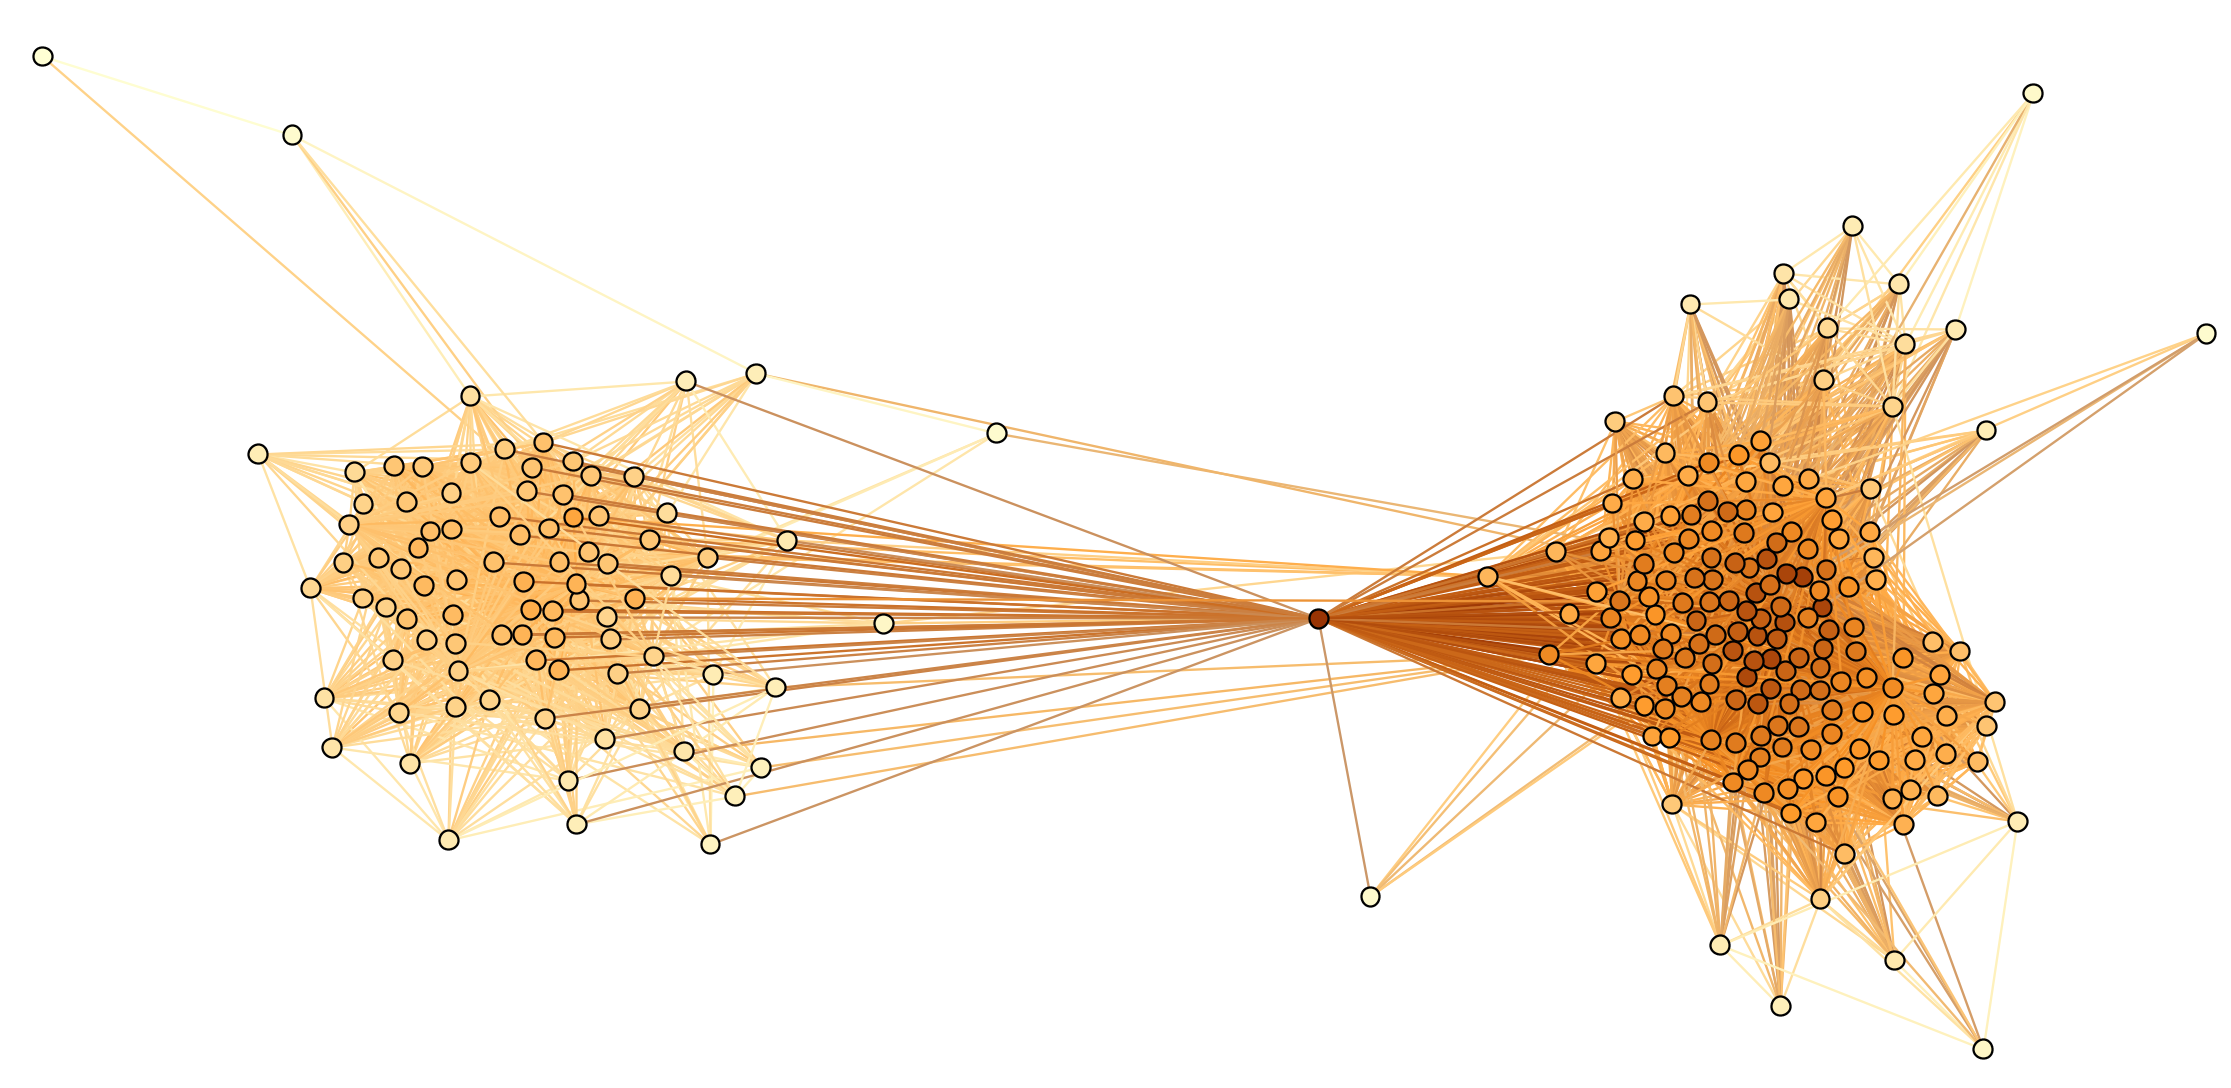
\includegraphics[scale=0.26]{facebook_1.png}
\end{center}
\end{frame}

\begin{frame}
\frametitle{페이스북 친구 네트워크}
\textbf{페이스북 네트워크 with Betweenness Centrality}
\begin{center}
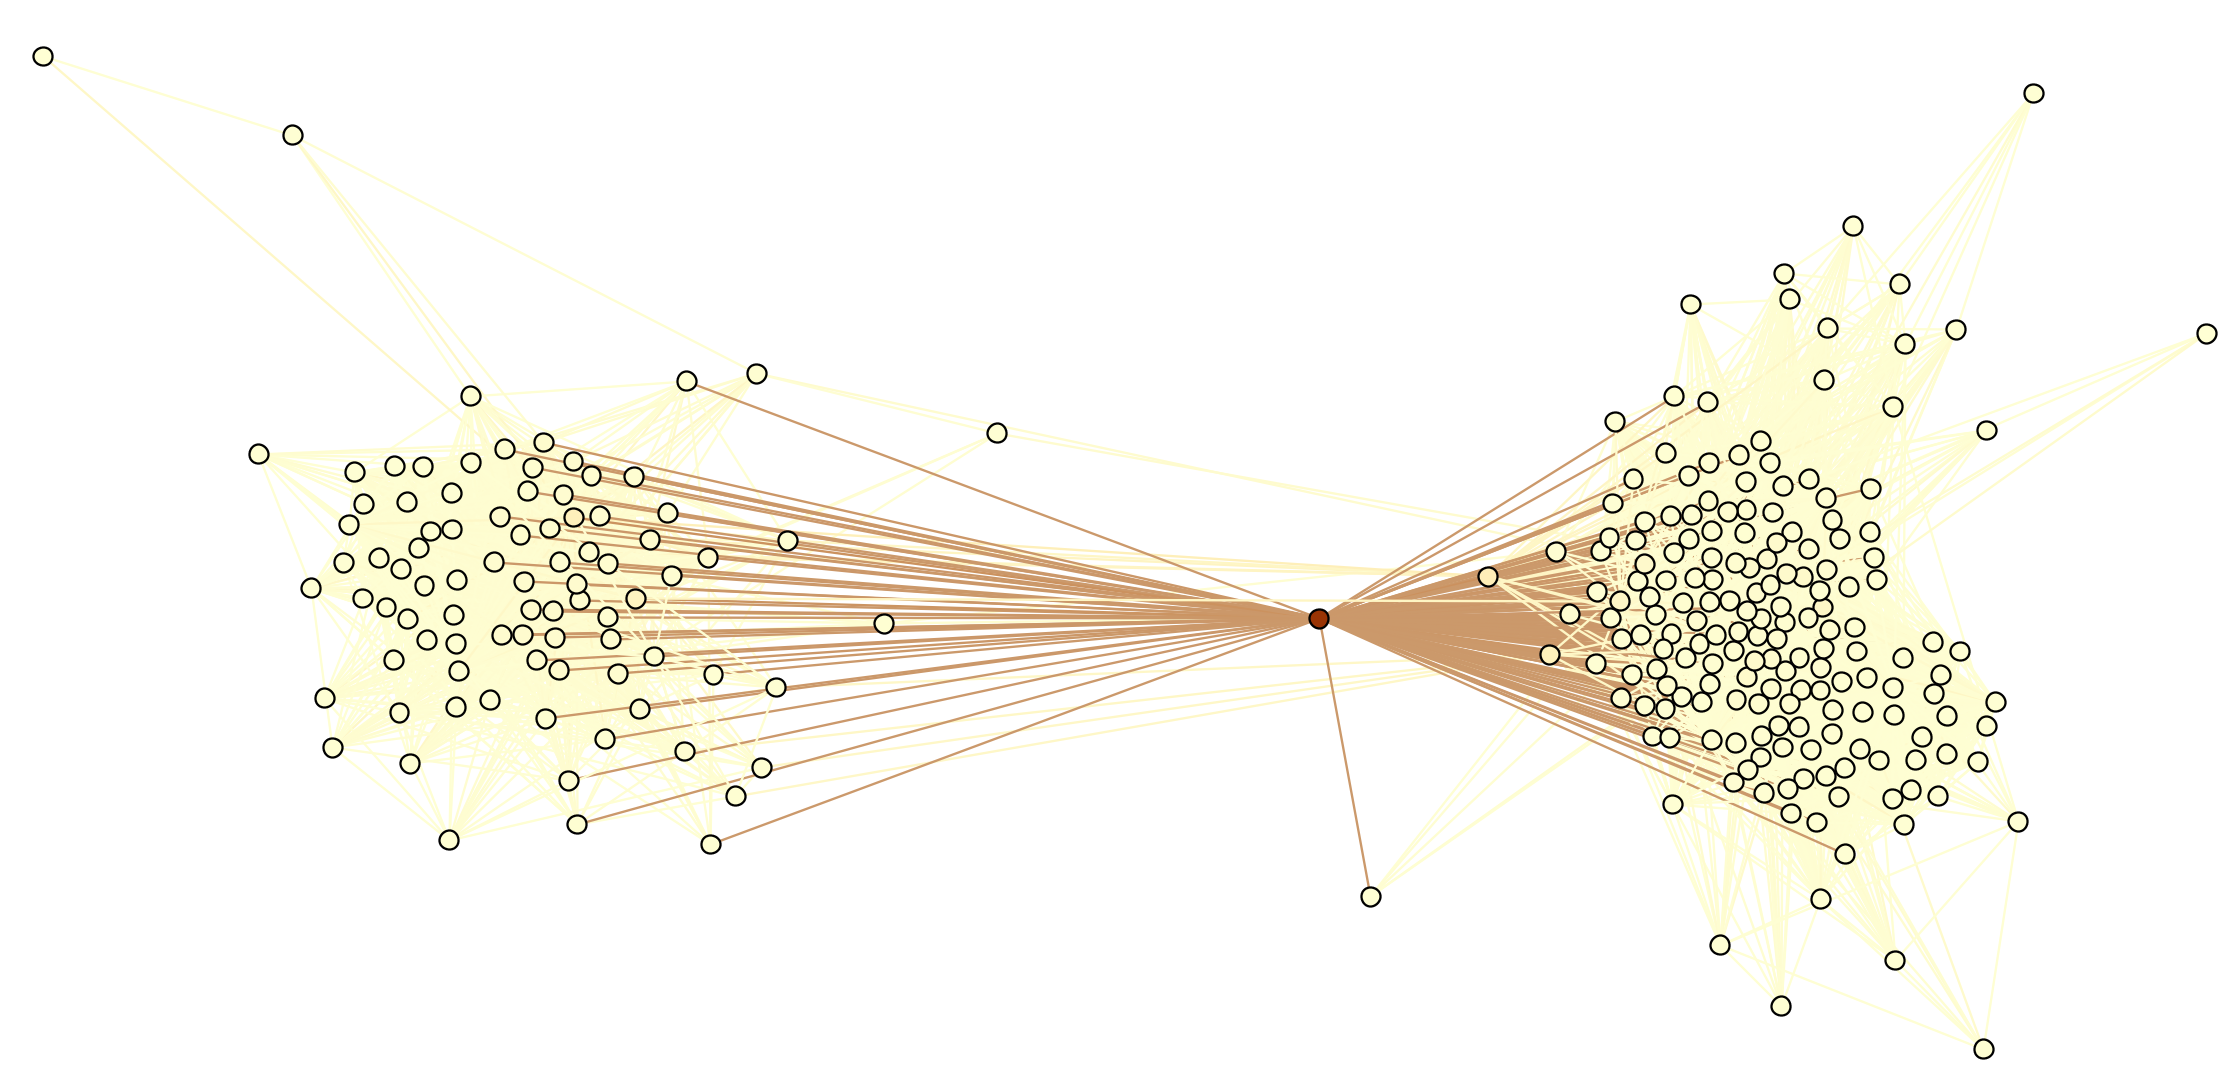
\includegraphics[scale=0.26]{facebook_2.png}
\end{center}
\end{frame}

%------------------------------------------------

\begin{frame}
\frametitle{Gephi로 네트워크 그리기}
\begin{center}
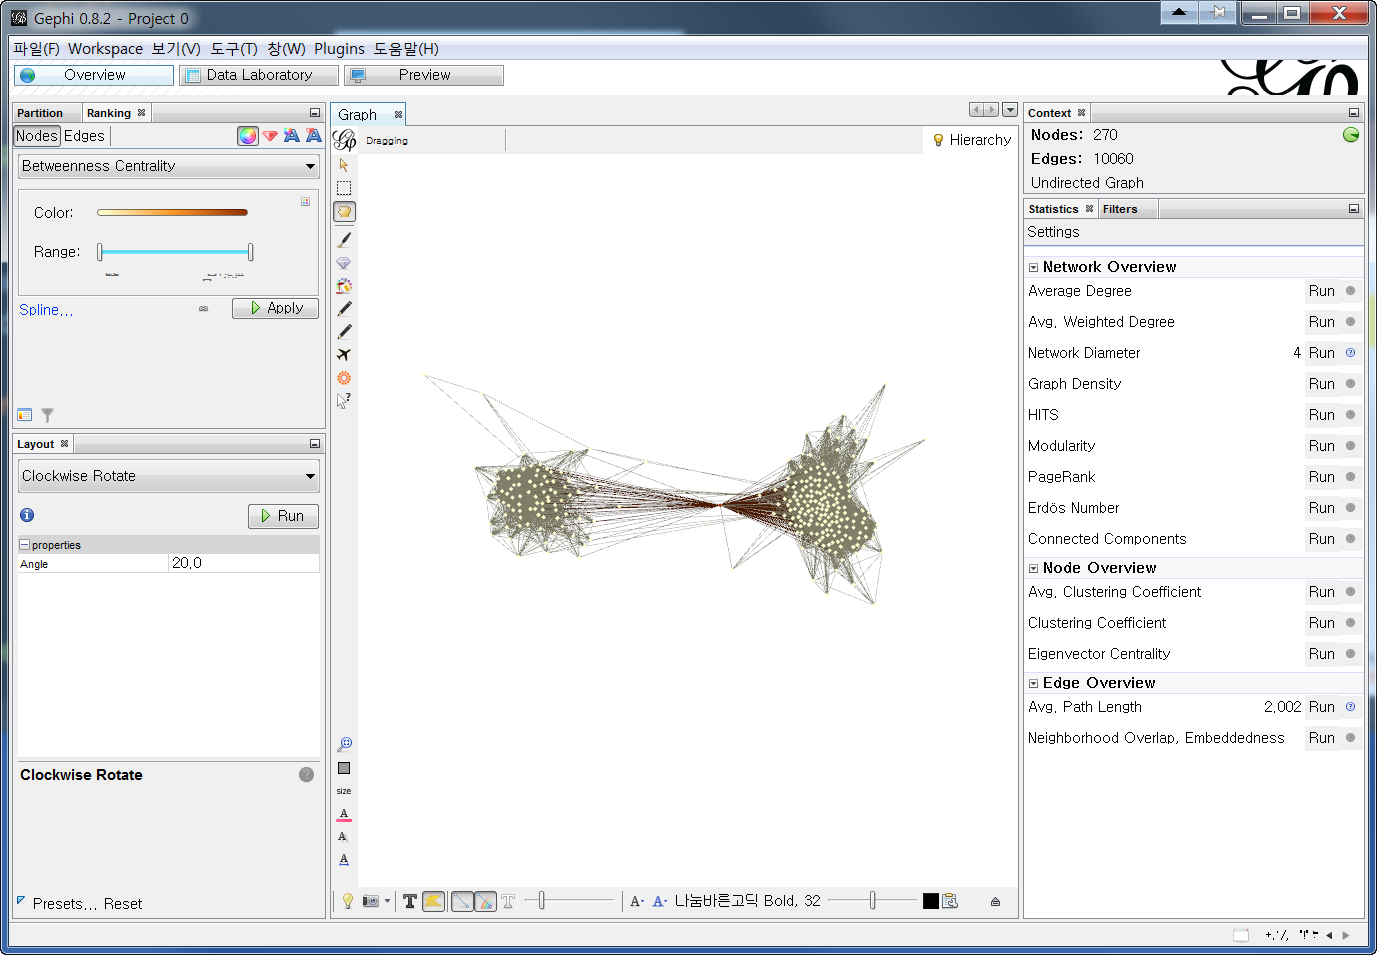
\includegraphics[scale=0.32]{gephi_2.png}
\end{center}
\tiny
{\color{blue}{\href{http://www.slideshare.net/koorukuroo/gephi-with-csv-file}{Gephi with CSV File}}}
\end{frame}
%------------------------------------------------
\section{기타 기능}
%------------------------------------------------
\begin{frame}[fragile]
\frametitle{기타 기능}
\begin{itemize}
\item 파일 내보내기
\item 파일 불러오기
\item 노드의 한글 표현 방법
\item 네트워크의 링크 예측
\end{itemize}
\end{frame}

\begin{frame}[fragile]
\frametitle{파일 내보내기}
\begin{block}{}
\begin{Verbatim}[numbers=left,commandchars=\\\{\}]
nx.write_graphml(G, `./graphfile.graphml')
nx.write_gexf(G, `파일 경로')
nx.write_gml
nx.write_yaml
nx.write_pajek
nx.write_shp
nx.dump # for JSON
\end{Verbatim}
\end{block}
\end{frame}

\begin{frame}[fragile]
\frametitle{파일 불러오기}
\begin{block}{}
\begin{Verbatim}[numbers=left,commandchars=\\\{\}]
nx.read_graphml(`./graphfile.graphml', unicode)
nx.read_gexf(G, `파일 경로')
nx.read_gml
nx.read_yaml
nx.read_pajek
nx.read_shp
nx.load # for JSON
\end{Verbatim}
\end{block}
\end{frame}



%------------------------------------------------
\begin{frame}[fragile]
\frametitle{노드의 한글 표현 방법}
\textbf{방법1. nx\_pylab.py의 수정}
\scriptsize
\begin{Verbatim}[numbers=left,commandchars=\\\{\}]
/usr/lib/pymodules/python2.7/networkx/drawing/nx_pylab.py
C:{\textbackslash}Anaconda32{\textbackslash}Lib{\textbackslash}site-packages{\textbackslash}networkx{\textbackslash}drawing{\textbackslash}nx_pylab.py

수정 방법 : \href{https://gist.github.com/koorukuroo/3aae9a3e900e868840ea}{https://gist.github.com/koorukuroo/3aae9a3e900e868840ea}
수정된 코드 : \href{https://gist.github.com/koorukuroo/5efb58a86c5396f13650}{https://gist.github.com/koorukuroo/5efb58a86c5396f13650}
\end{Verbatim}
\vspace{5mm}
\scriptsize
\textbf{사용방법}
\begin{Verbatim}[numbers=left,commandchars=\\\{\}]
import matplotlib.font_manager as fm
fp1 = fm.FontProperties(fname="{\color{blue}{./NotoSansKR-Regular.otf}}") 
# 무료 폰트 {\tiny{\href{https://www.google.co.kr/get/noto/#/}{https://www.google.com/get/noto/pkgs/NotoSansKorean-windows.zip}}}
nx.set_fontproperties(fp1)
{\color{red}{G = nx.Graph()}}
\end{Verbatim}
\end{frame}

\begin{frame}[fragile]
\frametitle{네트워크의 링크 예측}
\begin{block}{}
	\begin{Verbatim}[numbers=left,commandchars=\\\{\}]
대구과학고등학교 2014 R&E
연구자 : 김요한, 김현, 유주형, 유준승, 한승원
	\end{Verbatim}
\end{block}
\begin{center}
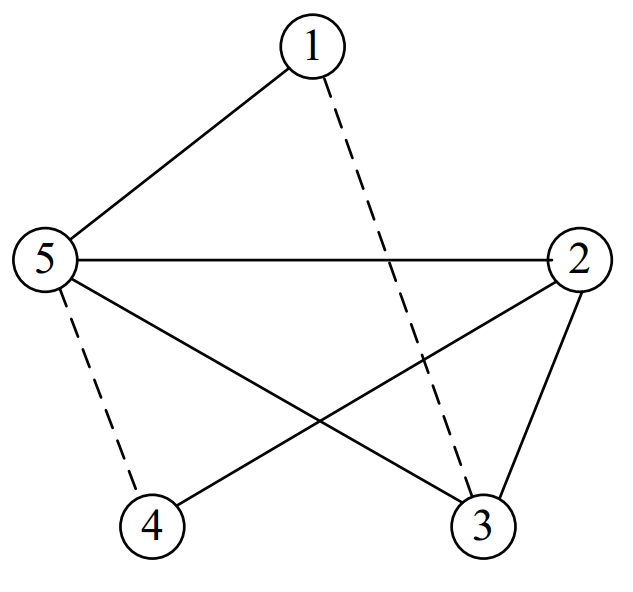
\includegraphics[scale=0.37]{prediction.png}
\end{center}
\tiny
\begin{Verbatim}
Lü, Linyuan, and Tao Zhou. "Link prediction in complex networks: A survey." Physica A(2011): 1150-1170.
\end{Verbatim}
\end{frame}

\begin{frame}[fragile]
\frametitle{네트워크의 링크 예측}
\begin{center}
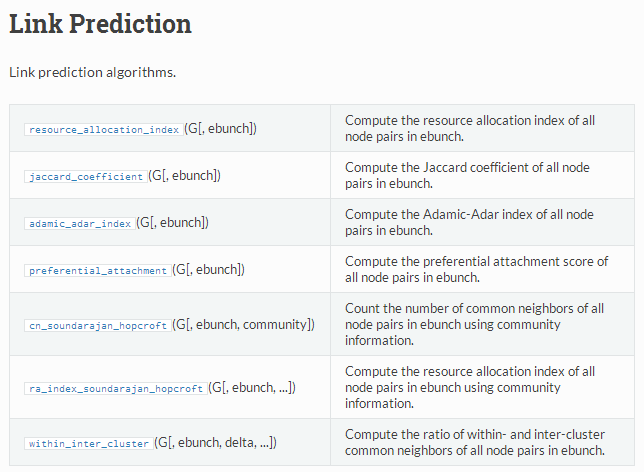
\includegraphics[scale=0.7]{link_prediction.png}
\end{center}
\end{frame}

\begin{frame}[fragile]
\frametitle{네트워크의 링크 예측}
\textbf{NetworkX 버전 업그레이드}
\scriptsize
\begin{block}{}
\begin{Verbatim}[numbers=left,commandchars=\\\{\}]
pip install --upgrade networkx==1.9
pip install --upgrade git+https://github.com/networkx/networkx.git#egg=networkx
\end{Verbatim}
\end{block}
{\color{blue}{\href{http://networkx.github.io/documentation/latest/install.html}{http://networkx.github.io/documentation/latest/install.html}}}\\
\vspace{2cm}
To be continue(?)
\end{frame}

\begin{frame}[fragile]
\frametitle{Appendix1. KLDP 개발자 네트워크}
\begin{center}
\href{http://dspace.kaist.ac.kr/handle/10203/21356}{
\includegraphics[scale=0.2]{kldp_1.png}}\\

\includegraphics[scale=0.25]{kldp_2.png}
\end{center}
\end{frame}

\begin{frame}[fragile]
\frametitle{Appendix1. KLDP 개발자 네트워크}
\begin{center}
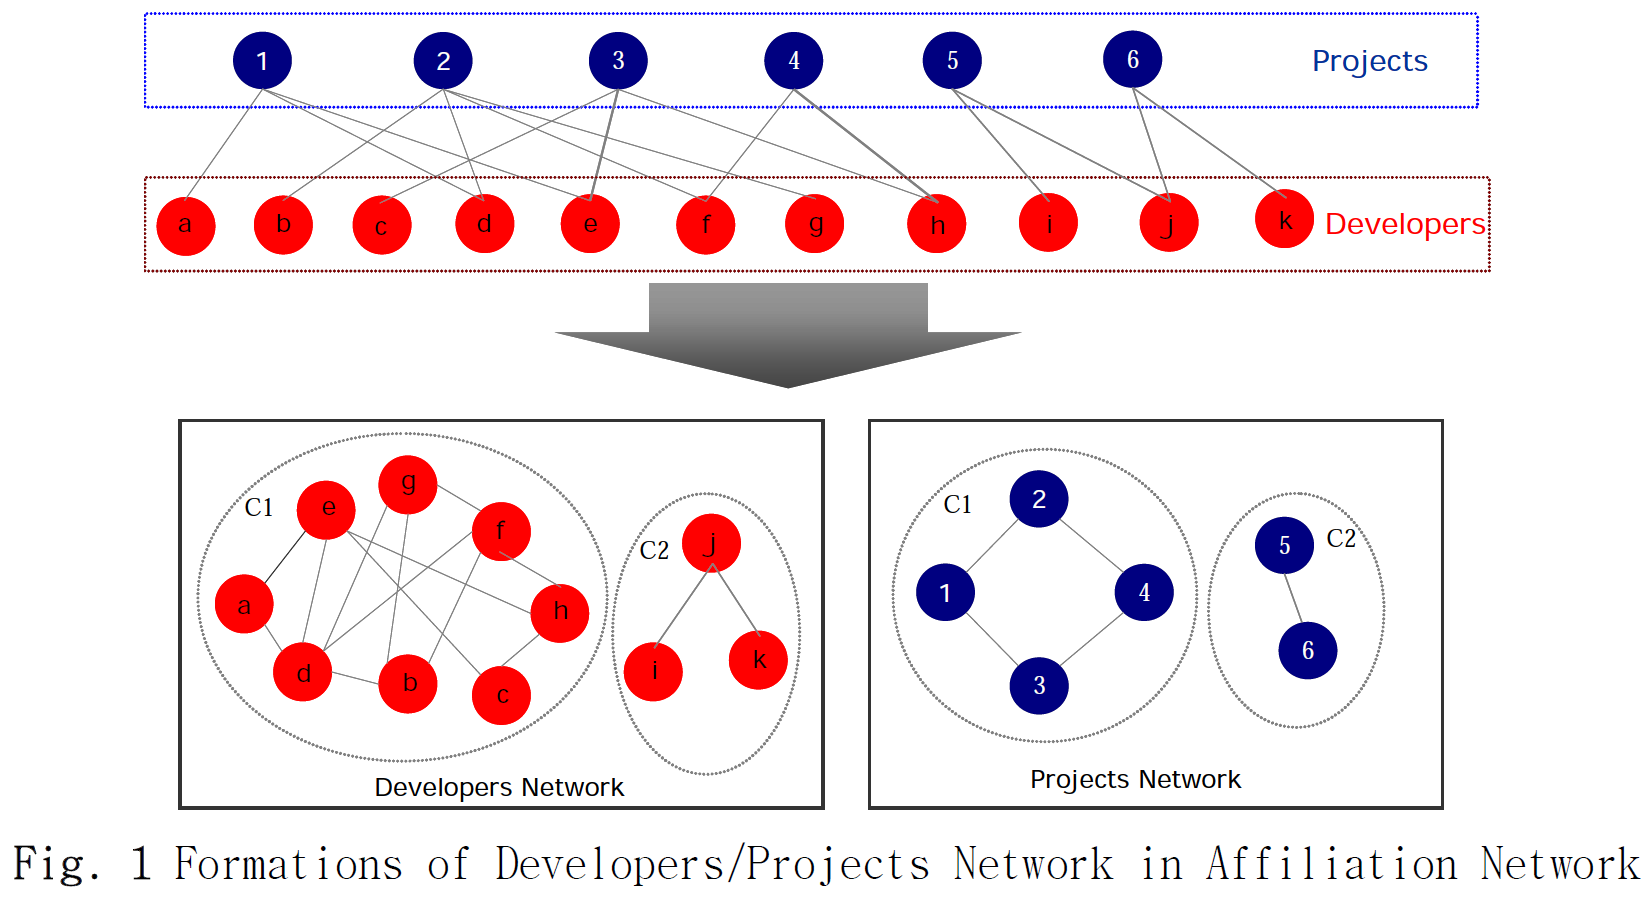
\includegraphics[scale=0.3]{kldp_3.png}
\end{center}
\hfill
\tiny{\href{http://dspace.kaist.ac.kr/handle/10203/21356}{http://dspace.kaist.ac.kr/handle/10203/21356}}
\end{frame}

\begin{frame}[fragile]
\frametitle{Appendix1. KLDP 개발자 네트워크}
\begin{center}
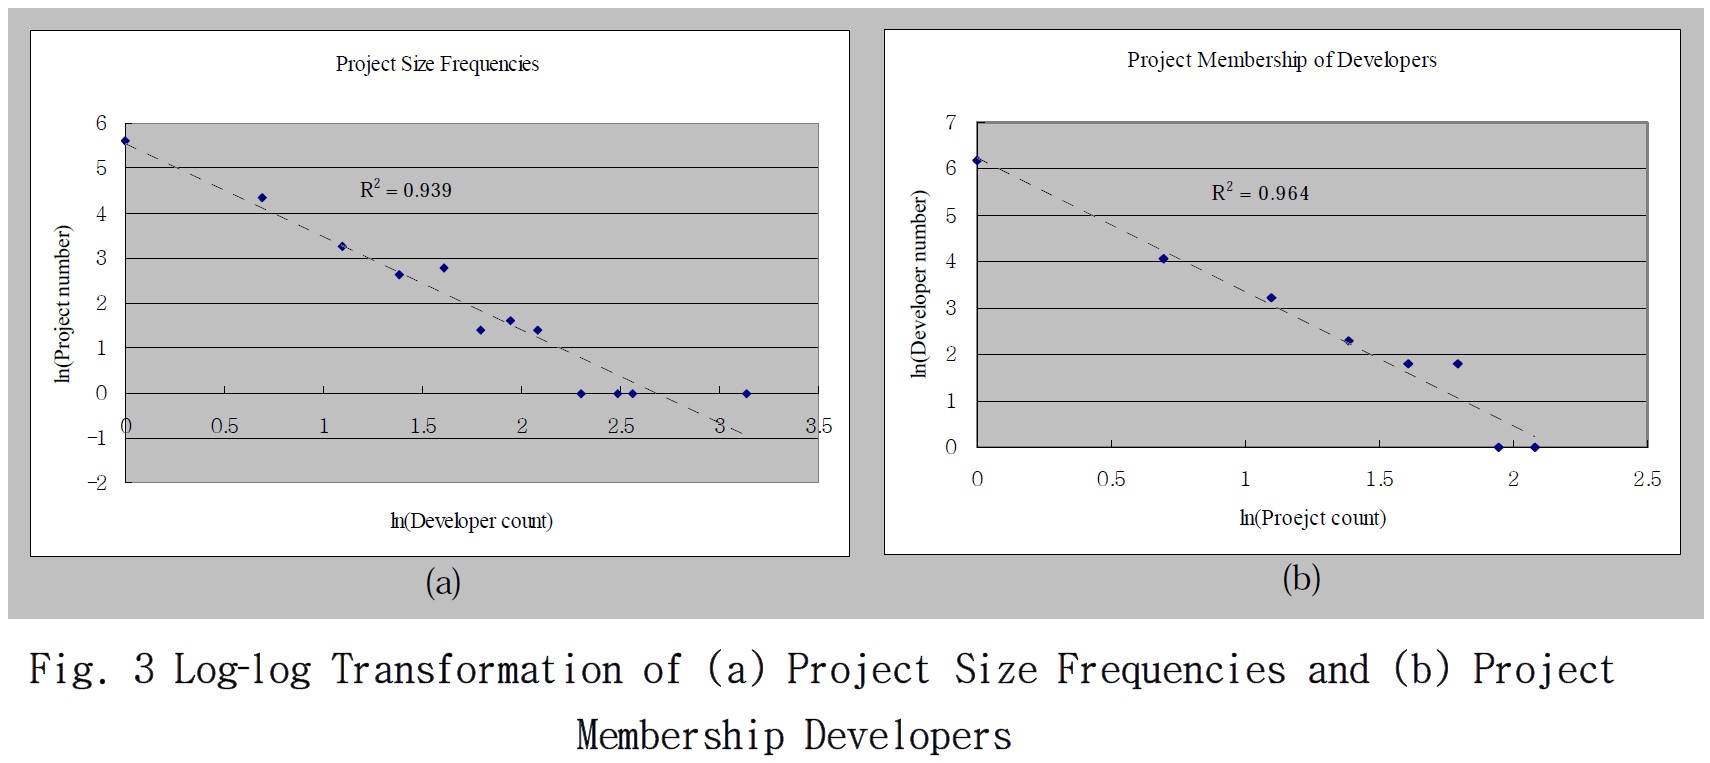
\includegraphics[scale=0.3]{kldp_4.png}
\end{center}
\hfill
\tiny{\href{http://dspace.kaist.ac.kr/handle/10203/21356}{http://dspace.kaist.ac.kr/handle/10203/21356}}
\end{frame}

\begin{frame}[fragile]
\frametitle{Appendix2. 점과 선의 체인지}
\begin{center}

\includegraphics[scale=0.23]{secretgarden.jpg}
\end{center}
\hfill
\tiny{SBS 시크릿가든 공식 홈페이지}
\end{frame}

\begin{frame}[fragile]
\frametitle{Appendix2. 점과 선의 체인지}
\begin{center}
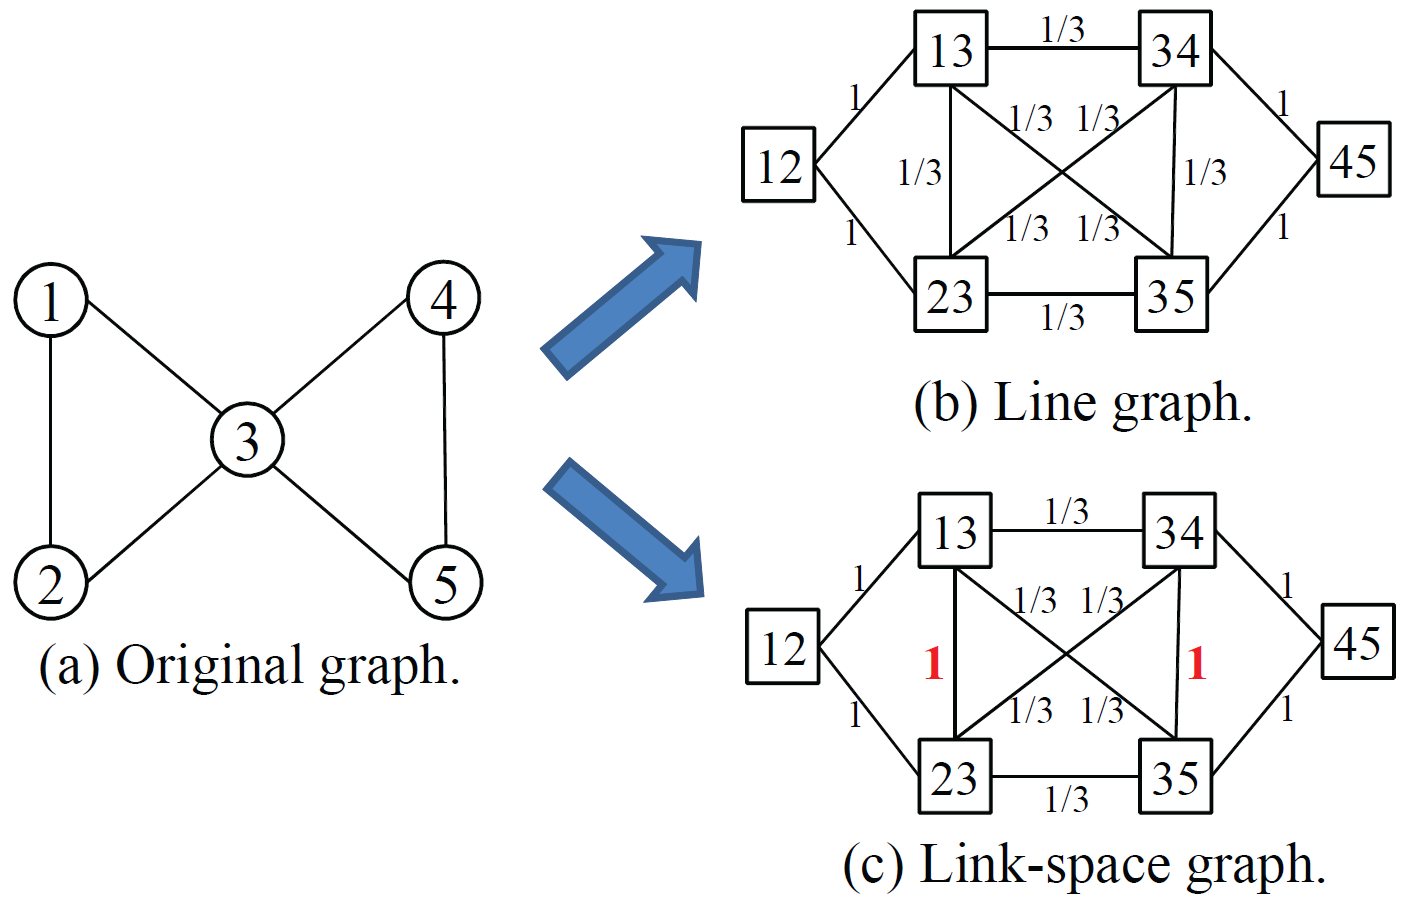
\includegraphics[scale=0.25]{linkscan.png}
\end{center}
\hfill
\tiny{
\begin{Verbatim}
Lim, Sungsu, et al. "LinkSCAN*: Overlapping community detection using the link-space transformation."
Data Engineering (ICDE), 2014 IEEE 30th International Conference on. IEEE, 2014.
\end{Verbatim}
}
\end{frame}

\begin{frame}[fragile]
\frametitle{Appendix3. Predict Ebola's Spread}
\begin{center}
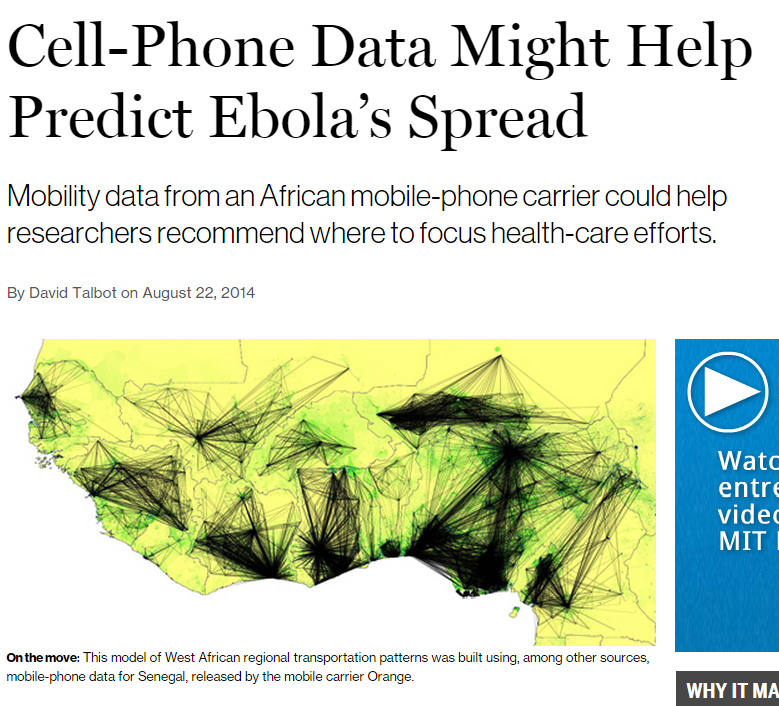
\includegraphics[scale=0.4]{ebolas.png}
\end{center}
\hfill
\tiny{\href{http://www.technologyreview.com/news/530296/cell-phone-data-might-help-predict-ebolas-spread/}{http://www.technologyreview.com/news/530296/cell-phone-data-might-help-predict-ebolas-spread/}}
\end{frame}

\begin{frame}
\frametitle{이번 TALK의 목적 (다시 확인)}
\begin{enumerate}
\item LaTeX\\

\includegraphics[scale=0.2]{donald.png}
\quad
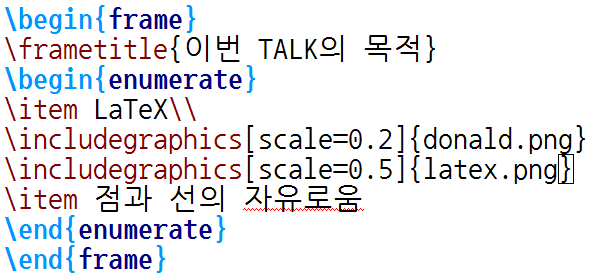
\includegraphics[scale=0.5]{latex.png}\\
\item 점과 선의 자유로움\\
\item 파이썬이라서 자유로운 점
\end{enumerate}
\end{frame}

{\fbckg{unist_scape.jpg}
\begin{frame}
\Huge{\centerline{The End}}
\end{frame}
}
%----------------------------------------------------------------------------------------

\end{document} 